\documentclass[]{article}

\usepackage[paperheight=18cm,paperwidth=14cm,textwidth=12cm]{geometry}
\usepackage[skip=20pt plus1pt, indent=40pt]{parskip}

\usepackage{graphicx}
\graphicspath{ {./images/} }
\usepackage{float}

\usepackage{amsmath}
\usepackage{amsfonts}
\usepackage{amssymb}

\usepackage{xcolor}
\usepackage{sectsty}
\definecolor{bittersweet}{rgb}{1.0, 0.44, 0.37}
\definecolor{grey}{rgb}{0.25, 0.25, 0.28}
\subsectionfont{\color{grey}}
\subsubsectionfont{\color{grey}}
\sectionfont{\color{bittersweet}}

\usepackage[T1]{fontenc}
\renewcommand\familydefault{\sfdefault} 

\usepackage{bm}

\newcommand{\ev}{\mathbb{E}[X]}
\renewcommand{\ev}[1]{\mathbb{E}[#1]}

\newcommand{\definizione}{\paragraph{Definizione:}}
\newcommand{\formula}{\paragraph{Formula generica:}}

\newcommand{\highlight}[1]{\colorbox{yellow}{$\displaystyle #1$}}

\begin{document}
    \tableofcontents
    \newpage
    \section{Introduzione alla probabilità}    
    \subsection{Glossario}
    \begin{itemize}
        \item Sistemi non deterministici $\rightarrow$ \textit{conoscendo i dati iniziali non possiamo determinare i dati finali}
        \item Incertezza degli eventi $\rightarrow$ \textit{la varianza degli eventi che possono succede}
        \item Rumore $\rightarrow$ \textit{possiamo misurare un evento solo approssimatamente}
        \item Probabilità $\rightarrow$ \textit{la materia che studia i sistemi non deterministici}
        \begin{itemize}
            \item Frequestista $\rightarrow $ \textit{probabilità assegnata sulla base di più esperimenti ripetuti nella stessa condizioni}
            \item Soggettivista $\rightarrow $ \textit{non esiste un valore oggettivo ma ci si basa sulla fiducia e sull'incertezza che l'individuo ha riguardo l'occorrenza di un certo evento}
        \end{itemize}
        \item Varianza $\rightarrow$ \textit{dispersione dei dati attorno al valore centrale / media / valore}
        \item Confidenza $\rightarrow$ \textit{intervallo che rappresenta una stima dei valori medi}
        \item Frequenza
        \begin{itemize}
            \item Frequenza assoluta $\rightarrow$ Numero di volte che si verifica un evento
            \item Frequenza relativa $\rightarrow$ Rapporto tra frequenza assoluta e il numero di prove/dati
        \end{itemize}
        \item Dataset $\rightarrow$ numero di dati a disposizione $\boldsymbol{D_n = \{ x_1 \ldots x_n \}} $
        \item Principio di enumerazione $\rightarrow$ Passare solo una volta da ogni elemento della raccolta
        \item Spazio esiti (s o $\Omega$) $\rightarrow$ Tutti i possibili esiti di un evento $\rightarrow$ $\boldsymbol{Dado=\{1 \ldots 6\}}$
        \item Spazio eventi (e) $\rightarrow$ Tutti i possibili risultati di un esperimento $\rightarrow$ $\boldsymbol{Dado=\{1||2\}} \leftarrow$ che esca \textbf{1} oppure \textbf{2}
        \item Assioma $\rightarrow$ Tre assiomi fondamentali su cui si poggia la teoria del calcolo delle probabilità
        \begin{itemize}
            \item 1' Assioma $\rightarrow$ La probabilità di E è un numero reale \textbf{non negativo} $\mathbb{P}(E) \in \mathbb{R}, \mathbb{P}(E) \geq 0$ $ \forall E \subseteq \Omega $ \space \textbf{|} \space $0 \leq P(E) \leq 1$
            \item 2' Assioma $\rightarrow$ Allo spazio degli esiti è sempre associato ad \textbf{1} \\ $\mathbb{P}(s) = 1$
            \item 3' Assioma $\rightarrow$ Per ogni coppia di eventi incompatibili $E_1, E_2 \subseteq \Omega$ \\ la probabilità di $E_1 \cup E_2$ è uguale alla \textbf{somma della loro probabilità} \\ $\mathbb{P}(E_1 \cup E_2) = \mathbb{P}(E_1) + \mathbb{P}(E_2)$
        \end{itemize} 
    \end{itemize}
    \newpage 

    \subsection{Moda e Mediana}
    \subsubsection{Moda}
    \definizione La moda è il valore che presenta la \textbf{massima frequenza} all'interno del dataset
    \formula
    \begin{equation*}
        Moda \rightarrow v_i : f_i = max f_i
        \begin{cases}
            \text{un solo valore} & \textbf{Moda} \\
            \text{più di un valore} & \textbf{Valori modali}
        \end{cases}
    \end{equation*}

    \subsubsection{Mediana}
    \definizione La mediana è il \textbf{valore centrale} all'interno del dataset (dati ordinati in ordine crescente/decresente)
    \formula
    \begin{equation*}
        Mediana =
        \begin{cases}
            \text{n pari} &  \frac{x_\frac{n}{2} + x_{\frac{n}{2}+ 1}}{2} \\
            \text{n dispari} & x_{[\frac{n+1}{2}]} \leftarrow \text{Intero superiore (Ceil)}
        \end{cases}
    \end{equation*}
    \paragraph{Esempio:} \[ D_n = \textbf{\{ 28, 34, 51, 19, 62, 43, 29, 38, 45, 26, 49, 33 \}} \]
    \paragraph{Per la mediana è necessario ordinare i dati in ordine crescente:} \[ D_n = \textbf{\{ 19, 26, 28, 29, 33, 34, 38, 43, 45, 49, 51, 62 \}} \]

    \[ \frac{x_{\frac{12}{2}} + x_{\frac{12}{2} + 1}}{2} = \frac{x_6 + x_7}{2} = \frac{34 + 38}{2} = \frac{72}{2} = \textbf{36} \]

    \paragraph{Nota:} quando si trova ad esempio $x_6$ bisogna andare a sostituire il valore con la posizione di x



    \subsection{Media e Varianza Campionaria}
    \subsubsection{Media Campionaria}
    \definizione La media campionaria è la \textbf{media} degli elementi di un campione.
    \formula  \[ \overline{X} = \frac{1}{n} \sum_{i=1}^{n} X_i \]

    \subsubsection{Varianza Campionaria}
    \definizione La varianza campionaria è la \textbf{dispersione} degli elementi di un campione.
    \formula \[ S^2 = \frac{\sum_{i = 1}^{n} (x_i - \overline{x})^2}{n-1} \]

    \paragraph{Esempio: (Varianza e Media)} $D_n = \textbf{\{ 3, 4, 6, 7, 10 \}}$ \\
    \linebreak[2]
 
    \text{Media del campione:} $ \overline{X} = \boldsymbol{\frac{( 3 + 4 + 6 + 7 + 10)}{5}} = \frac{30}{5} = 6 $ \\

    \text{Varianza campionaria:} $ s^2 = \boldsymbol{\frac{[ (-3)^2 + (-2)^2 + 0^2 + 1^2 + 4^2 ]}{4}} = 7.5 $ 

    \subsection{Disugaglianza di Chebyshev}
    \definizione Dice quanti dati di un campione cadono all'interno di un intervallo con centro la \textbf{media}

    \[ \forall k \geq 1 : k \in \mathbb{R} \]
    \[ (\overline{x} - k_s, \overline{x} + k_s) \longrightarrow \boldsymbol{S_k : [i : 1 \leq i \leq n, |x_i - \overline{x} < k_s|]} \]
    \paragraph{Generalizzando:}
    \[ |x - \overline{x}| < 5 \longrightarrow 68\% \]
    \[ |x - \overline{x}| < 25 \longrightarrow 95\% \]
    \[ |x - \overline{x}| < 35 \longrightarrow 99.7\% \]
    \subsection{Percentile}
    \definizione Il percentile è un indicatore che serve ad \textbf{indicare il valore minimo} sotto al quade ricade una \textbf{determinata percentuale} degli altri elementi sotto osservazione.
    \begin{equation*}
        Valore
        \begin{cases}
            \geq & \text{k \% dati} \\
            \leq & \text{100 - k \% dati}
        \end{cases}
    \end{equation*}
    \text{Prima cosa da fare è ordinare i valori in ordine crescente} \\
    \linebreak[3]
    \text{Dove il secondo quartile è sempre uguale alla \textbf{mediana}}
    \paragraph{Esempio:} $D_n = \textbf{\{ 0, 1, 2, 3, 4, 5, 6, 7, 8 \}}$

    \subsection{Insieme di dati Bivariati}
    \definizione è lo studio della relazione di due variabili.
    \formula \[ D_n : \{(X_1, Y_1) (X_2, Y_2) \ldots (X_n, Y_n)\}\]

    \subsubsection{Coefficiente di correlazione campionario}
    \definizione utilizzato per capire se esiste un legame \textbf{lineare} tra due serie di dati.
    \formula 
    \begin{equation*}
        r = \frac{\sum_{i = 1}^{n}(x_i - \overline{x}) (y_i - \overline{y})}{(n-1) s_x s_y} = \frac{\sum_{i = 1}^{n} (x_i - \overline{x}) (y_i - \overleftarrow{y})}{\sqrt{\sum_{i = 1}^{n} (x_i - \overline{x})^2 \sum_{i = 1}^{n} (y_i - \overline{y})^2}}
    \end{equation*}
    \subsection{Permutazioni, Combinazioni e Disposizioni}
    \subsubsection{Permutazioni}
    \definizione Modi possibili per sistemare \textbf{n} oggetti (\textbf{0! = 1})
    \[ n! = n \cdot (n-1) \ldots (n \cdot (n-1)) \]
    \paragraph{Esempio:} Fattoriale di 6
    \[ 6! = 6 \cdot (6-1) \cdot (6-2) \ldots (6-5) = 720 \]

    \subsubsection{Combinazioni}
    \definizione Modi di disporre \textbf{k} elementi scelti da \textbf{n} elementi (l'ordine \textbf{non conta})
    \[ \frac{n!}{k! \cdot (n-k)!} = \binom{n}{k} \]

    \paragraph{Esempio:} in una classe di \textbf{26} alunni si devono eleggere \textbf{2} rappresentanti
    \[ C_{n,k} = \frac{n!}{k! \cdot (n-k)!} \]
    \text{Sostituiamo \textbf{n} con \textit{26} (numero di alunni) e \textbf{k} con \textit{2} (numeri di rappresentanti)}
    \[ C_{26,2} = \frac{26!}{2! \cdot (26-2)!} = \frac{26!}{2! \cdot 24!} = \frac{25 \cdot 26}{2} = \textbf{325} \]
    \begin{center} 
        \text{è possibile anche semplificare i fattoriali come in questo caso}
    \end{center}

    \subsubsection{Disposizioni}
    \definizione Modi di disporre \textbf{k} elementi scelti da \textbf{n} elementi (l'ordine \textbf{conta})
    \[ \frac{n!}{(n-k)!}\]
    \paragraph{Esempio:} Quante parole is possono ottenere usando 4 \textbf{diverse} lettere da \textit{youmath} 
    \text{In questo caso dobbiamo contare le \textbf{disposizioni} senza ripetizione di \textbf{classe 4 di 7}}
    \[ D_{7,4} = \frac{7!}{(7-4)!} = \frac{7!}{3!} = \frac{5040}{6} = \textbf{840} \]



    \subsection{Probabilità condizionata}
    \definizione è la probabilità che succeda un evento \textbf{E} dato un evento \textbf{F}
    \[ P(E | F) = \frac{P(E | F)}{P(F)}\]
    \paragraph{Esempio:} \textbf{3} \text{scatole con contenuto nascosto dove in una è presente il premio} \\
    \[ P(Vincita) = \frac{1}{3}\]
    \[ P(Vincita | \text{1' pacco contiene un gatto}) = \frac{1}{2}\]
    \[ P(Vincita | \text{1' pacco \textbf{NON} contiene un gatto}) = 0\]



    \subsubsection{Teorema di Bayes}
    \formula \[ P(F_j | E) = \frac{P(F_j \cap E)}{P(E)} = \frac{P(E | F_j) \cdot P(F_j)}{\sum_{i = 1}^{p} P(E | F_i) \cdot P(F_i)} \]
    \begin{center} 
        \text{Probablità di \textbf{$F_j$} sapendo che si sia verificato l'evento \textbf{E}}
    \end{center}

    \subsection{Operazioni e proprietà tra eventi}
    \definizione Prendiamo come esempio \textbf{E} ed \textbf{F} come eventi
    \begin{itemize}
        \item E $\cup$ F $\longleftarrow$ Unione
        \item E $\cap$ F $\longleftarrow$ Intersezione
        \item E $\subset$ F | E $ \subseteq $ F $\longleftarrow$ Contenuto 
        \item E $\supset $ F | E $ \supseteq $ F $\longleftarrow$ Contiene
        \item $E^c$ $\longleftarrow$ Complemento
    \end{itemize}
    \paragraph{Le seguenti operazioni possono essere combinate tra di loro:} formando cosi le proprietà che seguono:
    \begin{itemize}
        \item $ E \cup (F \cup G) = (E \cup F) \cup G \longrightarrow$ Associativa unione
        \item $ (E \cup F) \cap G = (E \cap G) \cup (F \cup G) \longrightarrow$ Distributiva intersezione
        \item $ E \cap (F \cap G) = (E \cap F) \cap G \longrightarrow$ Associativa intersezione
        \item $ (E \cap F) \cup G = (E \cup G) \cap (F \cup G) \longrightarrow$ Distributiva unione
        \item $ (E \cup F)^c = \frac{E^c \cap F^c}{(E \cap F)^c} = E^c \cup F^c $
    \end{itemize}

    \section{Variabile aleatorie}
    \definizione La variabile aleatoria è una variabile che può assumere \textbf{valori diversi} \\ 
    in dipendenza da \textit{qualche esperimento casuale}.
    \[
        X
        \begin{cases}
            Discrete & \text{Solo \textbf{valori finiti}} \\
            Continue & \text{Possono assumere \textbf{range illimitati}}
        \end{cases}
    \]
    \subsection{Funzione di ripartizione (Tutte le variabili)}
    \definizione
    \text{La Probabilità che la variabile aleatoria \textbf{X} assuma un valore minore o uguale ad x}
    \formula $ F(x) = P(X \leq x) $
    \begin{itemize}
        \item F = funzione di ripartizione
        \item X = variabile aleatoria
        \item x = variabile normale
    \end{itemize}
    
    \paragraph{Esempio}:  \\
    \linebreak[4]
    $ P(a < X \leq b) $ \\
    \linebreak[4]
    $ P(X \leq b) = P(X \leq a) + P(a < X \leq b) $ \\
    \linebreak[4]
    $ P(a < X \leq b) = P(X \leq b) - P(X \leq a) = F(b) - F(a) $
    
  
    \subsection{Funzione di massa (Variabili discrete)}
    \formula $p(a) = P(X = a) $ \\
    \linebreak[4]
    \text{se si ha la funzione di ripartizione è possibile ottenere la funzione di massa perche:}
    \[ X \leq a = \cup X_i \]
    \formula \[ F(x) = P(X \leq a) = \sum_{x \leq a}^{} p(x_i) \]
    TODO- GRAFICO
    \paragraph{Esempio:} \text{variabile aleatoria X che può assumere valori \textbf{1}, \textbf{2} o \textbf{3}} \\
    \text{Dato che p(1) + p(2) + p(3) = \textbf{1}}
    \paragraph{Se:}
    \begin{minipage}{0.45\textwidth}
        \[ p(1) = \frac{1}{2} \]
    \end{minipage}
    \begin{minipage}{0.45\textwidth}
        \[ p(2) = \frac{1}{3} \]
    \end{minipage}
    
    \paragraph{Allora:}
    \[ p(3) = \frac{1}{6}\]

    \text{La funzione di ripartizione F di X è data da:}
    \begin{equation*}
        F(a) = \\
        \begin{cases}
            0 & a < 1 \\
            \frac{1}{2} & 1 \leq a < 2 \\
            \frac{5}{6} & 2 \leq a < 3 \\
            1 & 3 \leq a
        \end{cases}
    \end{equation*}

    \subsection{Funzione della densità di probabilità (Variabili continue)}
    \formula
    \[ P(X \in B) = \int_{B}^{} f(x) \,dx \]
    \[ P(X \in (-\infty, +\infty)) = \int_{-\infty}^{+\infty} f(x) \,dx=1 \]
    integrando $-\infty \text{ a} +\infty$ la probabilità che avvenga x è per forza 1 perche andiamo ad includere tutti i valori di $\mathbb{R}$

    \begin{center}
        \text{Se abbiamo che \textbf{B = [a, b]}} $\longrightarrow P(a \leq X \leq b) = \int_{a}^{b} f(x) \, dx $
        \\
        \text{Se abbiamo che \textbf{B = [a]}} $\longrightarrow P(X = a) = \int_{a}^{a} f(x) \, dx = 0 $
    \end{center}
   

    \text{Relazione che lega la funzione di ripartizione \textbf{F} alla densità \textbf{f}:}
    \[ F(x) = P(X \leq x) = \int_{-\infty}^{x} f(x )\, dx \]

    \text{Derivando entrambi i membri otteniamo che:}
    \[ \frac{d}{da} F(a) = f(a)  \]
    \paragraph{Esempio:} Sia assegnata una variabile aleatoria X con densità data da:
    \begin{equation*}
        f(x) = \\
        \begin{cases}
            C(4x - 2x^2) & 0 < x < 2 \\
            0 & \text{altrimenti}
        \end{cases}
    \end{equation*}
    \text{\textbf{(a)} quanto vale C? \textbf{(b)} quanto vale P(X > 1)? } \\
    \linebreak[4]
    \text{\textbf{(a)} siccome f è una densita allora:}
    \begin{equation*}
        \begin{split}
            1 & = C \int_{0}^{2} (4x - 2x^2) \, dx\\
            & = C[2x^2 - \frac{2x^3}{3}] \bigg\rvert_{x=0}^{x=2} = C \cdot \frac{8}{3} \\
            & = C = \frac{3}{8}
        \end{split}
    \end{equation*} \\
    \linebreak[4]
    \text{\textbf{(b)} conoscendo ora la densità f possiamo trovare la P(X > 1):}
    \[ P(X > 1) = \int_{1}^{\infty} f(x) \, dx = \frac{3}{8} \int_{1}^{2}(4x - 2x^2) \, dx = \frac{1}{2} \]
    \newpage

    \section{Funzioni a due variabili}
    Questo tipo di funzioni ci sono utili quando l'utilizzo di una sola variabile è impossibile poichè 
    \textit{l'oggetto in questione è basato sulla relazione di due variabili aleatorie}
    \subsection{Funzione di ripartizione congiunta}
    \definizione Funzione di ripartizione a due variabili aleatorie X e Y
    \formula \[ F(x, y) = P(X \leq x, Y \leq y) \]
    \text{Se vogliamo trovare solamente la funzione di ripartizione di una singola variabile aleatoria:}
    \begin{equation*}
    \begin{split}
        F_X(x) & = P(X \leq x) \\
        & = P(X \leq x, Y \leq \infty) \\
        & = F(x, \infty) \\
    \end{split}
    \end{equation*}
    Applicabile anche alla $F_y(y)$
    \[ F_Y(y) = F(\infty, y) \]

    \subsection{Funzione di massa congiunta}
    \definizione Probabilita che accadano due eventi (\textbf{X} e \textbf{Y}) nello stesso istante.
    \formula $ p(x_i, y_j) = P(X=x_i, Y=y_j) $

    \text{Se vogliamo trovare solamente la funzione di massa di una singola variabile aleatoria:}
    \begin{equation*}
        \begin{split}
            p_X(x_i) & := P(X = x_i) \\ 
            & = P(\underset{j}{\cup} \{ X=x_i, Y=y_j \}) \\
            & = \sum_{j}^{} P(X=x_i, Y=y_j) \\ 
            & = \sum_{j}^{} p(x_i, y_j) \\
        \end{split}
    \end{equation*}
    Applicabile anche alla $p_Y$
    \[ p_Y(y_j) = \sum_{i}^{} p(x_i, y_j) \]
    \linebreak[4]
    \[ \sum_{x}^{} \sum_{y}^{} p(x, y) = 1 \]

    \newpage
    \subsection{Funzione densità congiunta}
    \definizione Due variabili aleatorie X e Y sono \textit{congiuntamente continue} se esiste un funzione non negativa f(x,y)
    definita per tutti gli x e gli y
    \formula
    \[ P((X,Y) \in C) = \int_{}^{} \int_{(x,y) \in C}^{} f(x,y) \, dx \, dy \] \\

    \text{se A e B sono sottoinsiemi qualsiasi di $\mathbb{R}$ e C:= A x B}
    \[ C:= {(x,y) \in \mathbb{R}^2 : x \in A, y \in B}\]
    \text{Possiamo riscrivere la funzione di ripartizione congiunta di X e Y come segue:}
    \begin{equation*}
        \begin{split}
            F(a,b) & = P(X \leq a, Y \leq b) \\
            & = P(X \in a, Y \in b) \\
            & = \int_{B}^{} \int_{A}^{} f(x,y) \, dx \, dy \\
            & = \int_{-\infty}^{a} \int_{-\infty}^{b} f(x,y) \, dx \, dy \\
        \end{split}
    \end{equation*}
    \paragraph{Esempio:} Siano X e Y due variabili aleatorie congiuntamente continue con densità
    di probabilità data da:
    \begin{equation*}
        f(x,y) =
        \begin{cases}
            2e^{-x} e^{-2y} & x > 0, y > 0 \\
            0 & altrimenti
        \end{cases}
    \end{equation*}
    Si calcolino \textbf{(a)} P(X > 1, Y < 1)
    \begin{equation*}
        \begin{split}
            P(X > 1, Y < 1) & = \int_{0}^{1} \int_{1}^{\infty} 2e^{-x} e^{-2y} \, dx \, dy \\
            & = \int_{0}^{1} 2e^{-2y} (\int_{1}^{\infty} e^{-x} \, dx) \, dy \\
            & = \int_{0}^{1} 2e^{-2y}\{ -e^{-x}\} \rvert_{x=1}^{\infty} \, dy \\
            & = e^{-1} \int_{0}^{1} 2e^{-2y} \, dy \\
            & = e^{-1}(1 - e^{-2})
        \end{split}
    \end{equation*}
    \centerline{In questo caso si è integrato prima in una variabile e poi nell'altra}

    \subsection{Variabili aleatorie indipendenti}
    \subsubsection{X,Y indipendenti}
    \definizione
    \text{Un evento su una variabile non influenza l'altra.}
    \formula Se soddisfano questa richiesta le variabili si dicono \textit{indipendenti} 
    \[ P(X \in A, Y \in B) = P(X \in A) P(Y \in B)\]

    Usando gli assiomi della probabilità è possibile dimostrare che la definizione di sopra è equivalente a:
    \[ P(X \leq a, Y \leq b) = P(X \leq a) P(Y \leq b)\]
    \[ \forall a,b \in \mathbb{R} \]
    \linebreak[3]

    Ovvero che la funzione di ripartizione congiunta sia il prodotto delle marginali:
    \[ F(a,b) = F_X(a) F_Y(b)\]

    \textbf{Funzione di massa:}
    \[ p(a,b) = p_X(a) p_Y(b) \]
    \[ P(X=a, Y=b) = P(X=a) P(Y=b)\]
    \paragraph{Dimostrazione:}
    \begin{equation*}
        \begin{split}
            P(X \in A, Y \in B) & = \sum_{x \in A}^{} \sum_{y \in B}^{} p(x, y) \\
            & = \sum_{x \in A}^{} \sum_{y \in B}^{} p_X(x) p_Y(y) \\
            & = \sum_{x \in A}^{} p_X(x) \sum_{y \in B}^{} p_Y(y) \\
            & = P(X \in A) P(Y \in B)
        \end{split}
    \end{equation*}

    \paragraph{Funzione di densità:}
    \[ f(x, y) = f_X(x) f_Y(y)\]
    \[ \forall x,y \in \mathbb{R} \]
    
    \paragraph{Esempio con variabili indipendenti continue e con stessa funzione di densità:}
    \begin{equation*}
        f_X(t) = f_Y(t) =
        \begin{cases}
            e^{-t} & t > 0 \\
            0 & altrimenti
        \end{cases}
    \end{equation*}
    Quale è la densità di probabilità della variabile aleatoria data dal rapporto X/Y
    \begin{equation*}
    \begin{split}
        F_{X|Y}(a) & = P(X | Y \leq a) \\
        & = \int_{(x,y)}^{}\int_{x \leq ay}^{} f(x, y) \, dx \, dy \\ 
        & = \int_{(x,y)}^{}\int_{x \leq ay}^{} f(x) f(y) \, dx \, dy \\ 
        & = \int_{0}^{\infty} \int_{0}^{ay} e^{-x} f(x) f(y)\, dx \, dy \\ 
        & = \int_{0}^{\infty} e^{-y}(\int_{0}^{ay} e^{-x}) \, dy \\
        & = \int_{0}^{\infty} e^{-y} (1-e^{-ay}) \, dy \\ 
        & = [-e^{-y} + \frac{e^{-(a+1)y}}{(a+1)}] \bigg\rvert_{0}^{\infty} \\ 
        & =  1 - \frac{1}{a+1} 
    \end{split}
    \end{equation*}
    La funzione di densità si ricava infine \textbf{derivando} la funzione di ripartizione
    \[f_{X|Y}(a) = \frac{d}{da}(1- \frac{1}{a + 1}) = \frac{1}{(a + 1)^2} a > 0 \]

    \newpage
    \subsection{Distribuzioni condizionate}
    \definizione La distribuzione condizionata di Y dato X è la probabilità di X quando è conosciuto il valore assunto da X. \\
    A ogni distribuzione condizionata è associato un valore atteso condizionato e una varianza condizionata
    \formula $P(E|F) = \frac{P(E \cap F)}{P(F)}$

    \subsection{funzione di massa condizionata (Discrete)}
    \formula
    \begin{equation*}
        \begin{split}
            p_{X|Y}(X | Y) & = P (X=x, Y=y) \\
            & = \frac{P(X=x, Y=y)}{P(Y=y)} \\
            & = \frac{p(X,Y)}{p_Y(x, y) > 0} 
        \end{split}
    \end{equation*}
    \[ \forall x, \forall y \text{ con } p_Y(y) > 0\]
    \linebreak[4]
    \text{Se y non è un valore possibile di Y, ovvero se P(Y = y) = 0, la quantità $p_{X|Y}(x|y)$ non è definita }
    
    \paragraph{Esempio:} Siano X e Y due variabili aleatorie discrete con funzione di massa congiunta p dato che: 
    \begin{center}
        \begin{minipage}{0.2\textwidth}
            $p(0,0) = 0.4$
        \end{minipage}
        \begin{minipage}{0.2\textwidth}
            $p(0,1) = 0.2$
        \end{minipage}
        \begin{minipage}{0.2\textwidth}
            $p(1,0) = 0.1$
        \end{minipage}
        \begin{minipage}{0.2\textwidth}
            $p(1,1) = 0.3$
        \end{minipage}
    \end{center}
    Calcolare la massa di X condizionata da Y = 1
    \[ P(Y = 1) = \sum_{x}^{} p(x, 1) = p(0,1) + p(1,1) = 0.5 \]
    \paragraph{Quindi:}
    \[ P(X = 0 | Y = 1) = \frac{p(0,1)}{P(Y = 1)} = \frac{2}{5} \]
    \[ P(X = 1 | Y = 1) = \frac{p(1,1)}{P(Y = 1)} = \frac{3}{5} \]
    Se X e Y sono variabili congiuntamente continue, non è possibile utilizzare la
    definizione di distribuzione condizionata valida per quelle discrete, infatti sappiamo
    che P(Y = y) = 0 per tutti i valori di y


    \subsection{funzione di densità condizionata (Continue)}
    \formula
    \[ f_{X|Y}(x | y) = \frac{f(x, y)}{f_Y(y)}\]
    Se X e Y sono congiuntamente continue e A è un sottoinsieme di numeri reali per ogni y si può definire:
    \[ P(X \in A | Y = y) := \int_{A}^{} f_{X|Y}(x | y) \, dx \]

    Notiamo che X e Y sono indipendenti allora:
    \begin{center}
        \begin{minipage}{0.45 \textwidth}
            $ f_{X|Y}(x,y) = f_X(x) $
        \end{minipage}
        \begin{minipage}{0.45 \textwidth}
            $ P(X \in A | Y = y) = P(X \in A) $
        \end{minipage}
    \end{center}


    \paragraph{Esempio:} è data la seguente densità congiunta di X e Y



    \begin{equation*}
        f(x,y) =
        \begin{cases}
            \frac{12}{5} x(2-x-y) & 0 < x < 1, 0 < y < 1 \\
            0 & altrimenti
        \end{cases}
    \end{equation*} \\
    \linebreak[2]
    Si calcoli la densità condizionata di X rispetto a Y = y per 0 < y < 1. \\
    Se questi due numeri sono compresi tra 0 e 1 abbiamo che:

    \begin{equation*}
        \begin{split}
            f_{X|Y}(x,y):&= \frac{f(x,y)}{f_Y(y)} \\
            & = \frac{f(x, y)}{\int_{-\infty}^{\infty} f(x', y) \, dx'} \\
            & = \frac{x(2-x-y)}{\int_{0}^{1} x'(2-x'-y) \, dx'} \\
            & = \frac{x(2-x-y)}{\frac{2}{3} - \frac{y}{2}} \\
            & = \frac{6x(2-x-y)}{4-3y}
        \end{split}
    \end{equation*}


    \newpage
    \section{Valore atteso}
    \definizione Rappresenta la media pesata dei valori di una variabile aleatoria

    \subsection{Funzione di massa (Discrete)}
    \[ \ev{X} := \sum_{i}^{} x_i P(X = x_i) \]
    Si può dire quindi che il valore atteso è anche detto \textit{media} di X oppure \textit{aspettazione}

    \paragraph{Esempio semplice:} Se X è una variabile aleatoria con funzione di massa
    \[ p(0) = \frac{1}{2} = p(1) \]
    Allora:
    \[ \ev{X} = 0 \cdot \frac{1}{2} + 1 \cdot \frac{1}{2} = \frac{0+1}{2} = \frac{1}{2}\]

    \paragraph{Esempio dado fair 6 facce $P(x_i = i) = \frac{1}{6}$}
    \[ \ev{X} = \sum_{i=1}^{6} i \frac{1}{6} = \frac{1}{6} \sum_{i=1}^{6} i = \frac{21}{6} = \frac{7}{2} = 3.5 \]
    Oppure:
    \[ \ev{X} := 1 \cdot \frac{1}{6} + 2 \cdot \frac{1}{6} + 3 \cdot \frac{1}{6} + 4 \cdot \frac{1}{6} + 5 \cdot \frac{1}{6} + 6 \cdot \frac{1}{6} = \frac{7}{2} = 3.5 \]
    \text{dove il risultato è la media dei valori che X può assumere}

    \paragraph{Se N è molto grande} allora \textbf{$N_i \approx N_p(x_i)$}
    \[ \sum_{i}^{n} x_i p(x_i) \approx \sum_{i}^{n} x_i \frac{n_i}{n}\]
    
    
    \subsection{Funzione di densità (Continue)}
    \formula \[ \ev{X} := \int_{-\infty}^{+\infty} x f(x) \, dx \]
    \paragraph{Esempio:} Siamo in attesa di una comunicazione che deve arrivare dopo le ore 17. \\
    a partire dalle 17 è una variabile aleatoria con funzione di densità data da:
    \begin{equation*}
        f(x) = \\
        \begin{cases}
            \frac{1}{1.5} & \text{se 0 < x < 1.5} \\
            0 & \text{altrimenti}
        \end{cases}
    \end{equation*}
    Il valore atteso del tempo che trascorre tra le 17 e il momento di arrivo della comunicazione è quindi:
    \[ \ev{X} = \int_{0}^{1.5} \frac{x}{1.5} \, dx = 0.75\]

    \subsection{Valore atteso di una funzione}
    \definizione è possibile calcolare il valore atteso di una funzione g(X) notando che essa stessa è una variabile aleatoria \\
    quindi si applicano le stesse proprietà, come segue: \\
    \linebreak[4]

    \begin{minipage}{0.45\textwidth}
        \text{Variabile discreta:}
        \begin{equation*}
            \ev{g(X)} = \sum_{i}^{} g(x_i) p(x_i)
        \end{equation*}
    \end{minipage}
    \hfill
    \begin{minipage}{0.45\textwidth}
        \text{Variabile Continua:}
        \begin{equation*}
            \ev{g(x)} = \int_{-\infty}^{+\infty} g(x) f(x) \, dx
        \end{equation*}
    \end{minipage}

    \paragraph{Esempio (discrete):} quanto vale il valore atteso del quadrato di una variabile X con le seguenti funzioni di massa?
    \begin{equation*}
        \begin{minipage}{0.3\textwidth}
            p(0) = 0.2
        \end{minipage}
        \begin{minipage}{0.3\textwidth}
            p(1) = 0.5
        \end{minipage}
        \begin{minipage}{0.3\textwidth}
            p(2) = 0.3
        \end{minipage}
    \end{equation*} \\
    Se poniamo $Y := X^2$ questa diventa una variabile che può assumere i valori $0^2$, $1^2$, $2^2$
    \[ p_Y(0) := P(Y = 0^2) = 0.2 \]
    \[ p_Y(1) := P(Y = 1^2) = 0.5 \]
    \[ p_Y(4) := P(Y = 2^2) = 0.3 \]
    Quindi:
    \[ \ev{X^2} = \ev{Y} = 0 \cdot 0.2 + 1 \cdot 0.5 + 4 \cdot 0.3 = 1.7 \]
    Oppure (utilizzando la proposizione delle variabili discrete)
    \[ \ev{X^2} = 0^2 \cdot 0.2 + 1^2 \cdot 0.5 + 2^2 \cdot 0.3 = 1.7\]

    \paragraph{Esempio (continue):} Il tempo – in ore – necessario per localizzare un guasto nell’impianto
    elettrico di una fabbrica è una variabile aleatoria X con funzione di densità
    \begin{equation*}
        f(x) =
        \begin{cases}
            1 & 0 < x < 1 \\
            0 & \text{altrimenti}
        \end{cases}
    \end{equation*}
    Se il danno economico provocato da una interruzione di x ore è $x^3$, qual è il valore
    atteso di questo costo? \\
    \paragraph{Applicando la proposizione della variabile continua} possiamo ottenere quanto segue:
    \[ \ev{X^3} = \int_{0}^{1} x^3 \, dx = \frac{1}{4} \]

    \subsection{Dimostrazioni}
    \text{Sia per discreto che per continuo si applicano le seguenti proprietà:}
    \[ \ev{aX+b} = a \ev{X} + b \]
    Se proviamo a ponere a = 0 scopriamo che:
    \[ \ev{b} = b \]
    Se proviamo a ponere b = 0 scopriamo che:
    \[ \ev{aX} = a \ev{X} \]
    Ovvero, il valore atteso di un fattore costante moltiplicato per una variabile aleatoria,
    è pari alla costante per il valore atteso della variabile aleatoria.

    \paragraph{Per caso discreto:}
    \begin{equation*}
        \begin{split}
            \ev{aX + b} & = \sum_{x}^{} (ax + b) p(x) \\
            & = a \sum_{x}^{} xp(x) + b \sum_{x}^{} p(x) \\
            & = a\ev{X} + b
        \end{split}
    \end{equation*}

    \paragraph{Per caso continuo:}
    \begin{equation*}
        \begin{split}
            \ev{aX + b} & = \int_{-\infty}^{+\infty} (ax + b) f(x) \, dx \\
            & = a \int_{-\infty}^{+\infty} xf(x) \,dx + b \int_{-\infty}^{+\infty} f(x) \, dx \\
            & = a\ev{X} + b
        \end{split}
    \end{equation*}

    \subsection{Momenti N-esimi nel valore atteso}
    \definizione se n = 1,2 ... n, la quantità $\ev{X^n}$ se esiste viene detta \textit{momento n-esimo} della variabile aleatoria X. \\
    \linebreak[4]
    \centerline{è possibile applicare le formule di prima, come segue:}
    \begin{equation*}
        \ev{X^n} =
        \begin{cases}
            \sum_{x}^{} x^n p(x) & \text{se X è discreta} \\
            \int_{-\infty}^{+\infty} x^n f(x) \, dx & \text{se X è continua}
        \end{cases}
    \end{equation*}

    \subsection{Valore atteso della somma di due variabili}
    \definizione è possibile applicare le formule viste sopra anche quando abbiamo due variabili aleatorie \\
    \linebreak[4]
    se in questo caso $\boldsymbol{\ev{g(X,Y)}}$ esiste allora: \\
    \begin{equation*}
        \ev{g(X,Y)} =
        \begin{cases}
            \sum_{x}^{} \sum_{y}^{} g(x,y) p(x,y) & \text{Se discreto} \\
            \int_{-\infty}^{+\infty} \int_{-\infty}^{+\infty} g(x,y) f(x,y) \, dx \, dy & \text{Se continuo}
        \end{cases}
    \end{equation*}
    \linebreak[4]
    % \[ X, Y -> g(X,Y) - \boldsymbol{g: \mathbb{R}^2 \rightarrow \mathbb{R}} \]
    \text{se $g(X,Y)$ come $\boldsymbol{g = X + Y}$ allora}
    \[ \ev{X + Y} = \ev{X} + \ev{Y} \]

    \paragraph{Dimostrazione caso discreto:}
    \begin{equation*}
        \begin{split}
            \ev{X + Y} &= \sum_{x}^{} \sum_{y}^{} (x + y) p(x, y) \\
            & = \sum_{x}^{} x \cdot [\sum_{j}^{} p(x_i, y_j)] + \sum_{x}^{} y \cdot [\sum_{i}^{} p(x_i, y_j)] \\
            & = \sum_{x}^{} xp_X(x) + \sum_{y}^{} yp_Y(y) \\
            & = \ev{X} + \ev{Y}
        \end{split}
    \end{equation*}

    \paragraph{Dimostrazione caso continuo:}
    \begin{equation*}
        \begin{split}
            \ev{X + Y} &= \int_{-\infty}^{\infty} \int_{-\infty}^{\infty} (x + y) f(x, y) \, dx \, dy \\
            & = \int_{-\infty}^{\infty} x [\int_{-\infty}^{\infty} f(x,y) \, dy] \, dx + \int_{-\infty}^{+\infty} y [ \int_{-\infty}^{+\infty} f(x,y) \, dx ] \, dy \\
            & = \int_{-\infty}^{\infty} x f_X(x) \, dx + \int_{-\infty}^{\infty} yf_Y(y) \, dy \\
            & = \ev{X} + \ev{Y}
        \end{split}
    \end{equation*}

    \paragraph{è possibile applicare la ricorsione per il numero di variabili aleatori}
    \begin{equation*}
        \begin{split}
            \ev{X + Y + Z} &= \ev{(X + Y) + Z} \\
            & = \ev{X + Y} + \ev{Z} \\
            & = \ev{X} + \ev{Y} + \ev{Z}
        \end{split}
    \end{equation*}

    \paragraph{In generale per ogni n}
    \[ \ev{X_1 + X_2 + \ldots + X_n} = \ev{X_1} + \ev{X_2} + \ldots \ev{X_n} \]


    \paragraph{Esempio: 2 dadi a 6 facce}
    \begin{equation*}
      \begin{split}
        \ev{X + Y} & = \ev{X} + \ev{Y} \\
        & = \sum_{i = 1}^{6} x_i p(x_i) + \sum_{i = 1}^{6} y_i p(y_i) \\
        & = \sum_{i = 1}^{6} x_i \frac{1}{6} + \sum_{i = 1}^{6} y_i \frac{1}{6} \\
        & = \frac{7}{2} + \frac{7}{2} = 7 
      \end{split}  
    \end{equation*}
    
    \centerline{Dove \textbf{7} è il valore atteso della somma dei due dadi.}
    Se vogliamo predire il valore di X possiamo scegliere un numero che sarà ugual ad X.
    L'errore che commeteremo sarà di $\boldsymbol{(X - c)^2}$ \\

    Se \boldsymbol{$c = \ev{X}$} l'errore sarà minimizzato $\boldsymbol{\mu := \ev{X}}$
    \[ \ev{(X - c)^2} \geq \ev{(X - \mu)^2}\]

    \section{Varianza}
    \definizione Indica di quanto i dati si discostano dalla media al quadrato \\
    \begin{minipage}{0.45\textwidth}
        \[ \mu = \ev{X} \leftarrow \text{Primo momento}\]
    \end{minipage}
    \begin{minipage}{0.45\textwidth}
        \[ \ev{X^2} \leftarrow \text{Momento secondo}\]
    \end{minipage}

    \formula \[ Var(X) := \ev{(X - \mu)^2} \]

    \paragraph{Generalizzazione:}
    \begin{equation*}
        \begin{split}
            Var(X) & = \ev{(X - \mu)^2} \\
            & = \ev{X^2 - 2 \mu \cdot X + \mu^2} \\
            & = \ev{X^2} - 2 \mu \cdot \ev{X} + \mu^2 \\
            & = \ev{X^2} - \mu^2 \longrightarrow \ev{X^2} - \ev{X}^2
        \end{split}
    \end{equation*}
    
    \paragraph{Esempio: Varianza di un dado}
    \begin{equation*}
        \begin{split}
            \ev{X^2} & = \sum_{1}^{6} i^2 P(X = i) \\
            & = 1^2 \cdot \frac{1}{6} + 2^2 \cdot \frac{1}{6} + 3^2 \cdot \frac{1}{6} + 4^2 \cdot \frac{1}{6} + 5^2 \cdot \frac{1}{6} + 6^2 \cdot \frac{1}{6} \\
            & = \frac{91}{6}
        \end{split}
    \end{equation*} \\

    Sapendo che $\ev{X} = \frac{7}{2}$
    \[ Var(X) = \ev{X^2} - \ev{X}^2 = \frac{91}{6} - (\frac{7}{2})^2 = \frac{35}{12} \]

    \subsection{Costanti reali nella varianza}
    Una utile identità che riguarda la varianza è la seguente (per ogni coppia di costanti reali a e b)
    \[ Var(aX + b) = a^2 \cdot Var(X) \] \\

    Per dimostrare ciò ricordiamoci sempre di $\boldsymbol{\mu := \ev{X}}$
    \paragraph{Dimostrazione:}
    \begin{equation*}
        \begin{split}
            Var(aX + b) :&= \ev{(aX + b - \ev{aX + b})^2} \\
            & = \ev{(aX + b -a\mu - b)^2} \\
            & = \ev{a^2(X-\mu)^2} \\
            & = a^2 \ev{(X - \mu)^2} \\
            & = a^2 Var(X)
        \end{split}
    \end{equation*}
    Se sostituiamo i valori di \textbf{a} e \textbf{b} troviamo che: \\
    SE $a = 0 \longrightarrow Var(b) = 0 \longrightarrow \text{le costanti hanno varianza \textbf{nulla}}$ \\
    SE $a = 1 \longrightarrow Var(X + b) = Var(X) \longrightarrow \text{sommando una const. non cambia la varianza}$ \\
    SE $b = 0 \longrightarrow Var(aX) = a^2 \cdot Var(X)$ \\
    

    \newpage
    \section{Deviazione Standard}
    \definizione Indica di quanto dei dati si \textbf{discotastano dalla media} (non al quadrato)

    \formula \[ S = \sqrt{Var(X)} \]

    \[ Var(X + X) = Var(2 \cdot X) = 4 \cdot Var(X) \]
    \linebreak[1]
    \textbf{Se X è indipendente allora:}
    \[ Var(X) + Var(X) = Var(X + X) \]

    \newpage
    \section{Covarianza}
    \definizione Misura la \textbf{variazione} tra due variabili aleatorie associate tra di loro
    \formula \[ \boldsymbol{Cov(X,Y) := \ev{(X - \mu_X) (Y - \mu_Y)}} \]
    \textbf{Dove:} \\
    $ \mu_x = \ev{X} $ \\
    $ \mu_y = \ev{Y} $ \\
    \linebreak[4]
    \centerline{\textit{La covarianza può essere negativa, positiva o nulla } }
    \text{\textbf{Positivo} $\longrightarrow$ Le due variabili crescono o decrescono insieme} \\
    \text{\textbf{Negativo} $\longrightarrow$ Quando una variabile cresce l'altra decresce} \\
    \text{\textbf{Nullo} $\longrightarrow$ Le due variabili sono indipendenti} \\

    è presente una formula alternativa \textbf{più semplice} \textit{(si trova espandendo il prodotto al secondo membro)}

    \begin{equation*}
        \begin{split} 
            Cov(X, Y) &= \ev{XY - \mu_XY - \mu_YX + \mu_X \mu_Y} \\
            & = \ev{XY} - \mu_X \ev{Y} - \mu_Y \ev{X} + \mu_X \mu_Y \\ 
            & = \ev{XY} - \mu_X \mu_Y - \mu_X \mu_Y  + \mu_X \mu_Y  \\
            & = \ev{XY} - \ev{X} \ev{Y}
        \end{split}
    \end{equation*}


    \subsection{Proprietà della covarianza}
    $ Cov(X, Y) = Cov(Y, X) \longleftarrow \text{Simmetria} $ \\ \\
    $ Cov(X, X) = Var(X) \longleftarrow \text{Generalizzazione della varianza} $ \\ \\
    $ Cov(X+Y, Z) = Cov(X, Z) + Cov(Y, Z) $ \\ \\
    $ Cov(X+Y, Z+W) = Cov(X, Z) + Cov(X, W) + Cov(Y, Z) + Cov(Y, W) $ \\ \\
    $ Var(X + Y) = Var(X) + Var(Y) + 2 Cov(X, Y) $ \\ \\
    
    \centerline{- Se $X_1 \ldots X_n$ e $Y $ sono variabili aleatorie qualsiasi allora:}
    \[ Cov(\sum_{i = 1}^{n}X_i, Y) = \sum_{i = 1}^{n} Cov(X_i, Y) \]

    \centerline{- Se $X_1 \ldots X_n$ e $Y_1 \ldots Y_m$ sono variabili aleatorie qualsiasi allora:}
    \[ Cov(\sum_{i = 1}^{n}X_i, \sum_{j = 1}^{m} Y_j) = \sum_{i = 1}^{n} \sum_{j = 1}^{m} Cov(X_i, Y_j) \] \\
    \linebreak[10]
    \centerline{Se X e Y sono variabili aleatorie \textbf{indipendenti:}}
    \[ \ev{XY} = \ev{X} \ev{Y} \]
    Questo implica che:
    \[ Cov(X, Y) = 0 \]

    \paragraph{Esempio:} varianza della somma di 10 lanci indipendenti di un dado \\
    Denotiamo con \textbf{$X_i$} il punteggio del dado \textit{i-esimo}, sappiamo che:
    \begin{equation*}
        \begin{split}
            Var(\sum_{i = 1}^{10} X_i) &= \sum_{i = 1}^{10} Var(X_i) \\
            & = 10 \cdot \frac{35}{12} \\
            & = \frac{175}{6}
        \end{split}
    \end{equation*}
    
    \subsection{Coefficiente di correlazione lineare}
    \definizione numero puro che tiene conto della deviazione standard di X e Y
    \formula
    \begin{equation*}
        Corr(X,Y) := \frac{Cov(X,Y)}{\sqrt{Var(X) \cdot Var(Y)}}
    \end{equation*}

    \begin{center}
        La correlazione può assumere valori compresi tra \textbf{-1} e \textbf{1}
    \end{center}
    \text{\textbf{-1} $\longrightarrow$ Le due variabili sono inversamente proporzionali} \\
    \text{\textbf{0} $\longrightarrow$ Le due variabili sono indipendenti} \\
    \text{\textbf{1} $\longrightarrow$ Le due variabili sono crescono o decrescono con lo stesso rapporto} \\

    \newpage
    \section{Funzione generatrice dei momenti}
    \definizione Funzione che ci permette di calcolare i momenti della distribuzione.
    \formula \[ \phi(t) = \ev{e^{tX}}\]

    \centerline{Dove X è una variabile aleatoria e t è un parametro reale}

    \begin{equation*}
        \phi(t) := \ev{e^{tX}} = 
        \displaystyle
        \begin{cases}
            \displaystyle \sum_{x}^{} e^{tx}p(x) & \text{se X discreta} \\
            \displaystyle \int_{-\infty}^{+\infty} e^{tx} f(x) \, dx & \text{se X continua}
        \end{cases}
    \end{equation*}
    \linebreak[10]
    Derivando la funzione si ottengono i momenti:
    \[ \phi'(t) = \frac{d}{dt} \ev{e^{tX}} = \ev{\frac{d}{dt} e^{tX}} = \ev{Xe^{tX} \longrightarrow \phi'(0) = \ev{X}}\]
    \linebreak[10]
    Analogamente:
    \[ \phi''(t) = \frac{d^2}{dt^2} \ev{e^{tX}} = \ev{\frac{d^2}{dt^2} e^{tX}} = \ev{X^2e^{tX} \longrightarrow \phi''(0) = \ev{X^2}}\]


    \paragraph{Generalizzando:}
    \[ \phi^{(n)}(0) = \ev{X^n} \]
    \linebreak[2]

    \begin{minipage}{0.45\linewidth}
        Media:
        \[\mu_x = \phi'(0)\]
    \end{minipage}
    \begin{minipage}{0.45\linewidth}
        Varianza:
        \[ \sigma^{2}_x = \phi''(0) = \{\phi(0)'\}' \]
    \end{minipage}

    \paragraph{Ipotizziamo:} se X e Y sono indipendenti con $\phi_X$ e $\phi_Y$ e se $\phi_{X + Y}$ \\
    è la funzione generatrice dei momenti di X + Y allora:
    \[ \phi_{X + Y}(t) = \phi_X(t) \phi_Y(t) \]

    \text{Concludiamo che:}
    \begin{equation*}
        \begin{split}
            \phi_{X + Y}(t) :&= \ev{e^{t(X + Y)}} \\
            & = \ev{e^{tX} e^{tY}} \\
            & = \ev{e^{tX}} \ev{e^{tY}} \\
            & = \phi_X(t) \phi_Y(t)
        \end{split}
    \end{equation*}
    


    \subsection{Disugaglianza di Markov}
    \definizione Ci permette di sapere la probabilità che una variabile assuma valori molto grandi \\
    Serve per calcolare che una variabile aleatoria assuma un minimo di "a" $\longrightarrow a \in \mathbb{R}$

    \paragraph{Solo per variabili positive:} $X \in (0, +\infty) $
    \formula \[ P(X \geq a) \leq \frac{\ev{X}}{a}\]

    \paragraph{Dimostrazione:}
    \begin{equation*}
        \begin{split}
            \ev{X} & := \int_{0}^{+\infty} xf(x) \, dx \\
            & = \int_{0}^{a} x f(x) \, dx + \int_{a}^{+\infty} x f(x) \, dx \\ 
            & \geq \int_{a}^{+\infty} x f(x) \, dx \\ 
            & \geq \int_{a}^{+\infty} a f(x) \, dx \\
            & = a \int_{a}^{+\infty} f(x) \, dx \\ 
            & = \boldsymbol{aP(X \geq a)}
        \end{split}
    \end{equation*}
    
    \subsection{Disugaglianza di Chebyshev}
    \definizione Ci permette di sapere la probabilità che una variabile si discosti dalla media per più di un certo numero di deviazioni standard.
    
    \begin{equation*}
        \text{Se} X \text{var aleatoria}
        \begin{cases}
            \mu & \text{Media} \\
            \sigma^2 & \text{Varianza}
        \end{cases}
    \end{equation*}

    \centerline{Per ogni \textbf{r > 0} $\longrightarrow$ valore che indica il discostamento dalla media}
    \formula 
    \[ P(|X - \mu| \geq r) \leq \frac{\sigma^2}{r^2} \]

    \paragraph{Dimostrazione:} Dimostriamo che: \\
    \begin{minipage}{0.45\linewidth}
        \[ \{ |X - \mu | \geq r \} \]
    \end{minipage}
    \begin{minipage}{0.45\linewidth}
        \[ \{ ( X - \mu )^2 \geq r^2 \} \]
    \end{minipage} \\
    \linebreak[4]
    Questi due eventi coincidono e quindi sono \textbf{equiprobabili} \\
    Sapendo per certo che \boldsymbol{$(X - \mu)^2$} è \textit{non negativa} \\
    Possiamo applicare \textbf{Markov} con $a = r^2$ ottenendo:

    \begin{equation*}
        \begin{split}
            P(|X - \mu | \geq r) & = P((X - \mu)^2 \geq r^2) \\
            & \leq \frac{\ev{(X - \mu)^2}}{r^2} = \frac{\sigma^2}{r^2}
        \end{split}
    \end{equation*}
    \linebreak
 
    La disuguaglianza di \textbf{Markov} e di \textbf{Chebyshev} servono per ottenere le stime di probabilità di eventi rari di variabili
    cui conosciamo solo la \textbf{media} e la \textbf{varianza}.

    \paragraph{Postilla:} in caso di \textit{distribuzione nota} non c'è bisogno di utilizzare una di queste disuguaglianze.

    \paragraph{Esempio:} I numeri di pezzi prodotti in una settimana è una X di \textbf{50} \\
    \textbf{(a)} Cosa si può dire sulla probabilità che la produzione superi i 75 pezzi (\textit{a})? \\ \\
    \textbf{(b)} Se è nota anche la varianza pari a \textbf{25} cosa si può dire sulla probabilità che la produzione sia compresa tra i \textit{40} e i \textit{60} pezzi? \\
    \linebreak[4]
    \textbf{(a)} per la disuglianza di \textit{Markov}
    \[ P(X \geq 75) \leq \frac{\ev{X}}{75} = \frac{50}{75} = \frac{2}{3}\]

    \textbf{(b)} Applicando la disuguaglianza di \textit{Chebyshev}
    \[ P(|X - 50| \geq 10) \leq \frac{25}{10^2} = \frac{1}{4}\]
    Quindi:
    \[ P(40 \leq X \leq 60) = P(|X - 50| \leq 10) \geq 1 - \frac{1}{4} = \frac{3}{4}\]

    Perciò la probabilità che la produzione sia compresa tra \textit{40} e i \textit{60} pezzi è almeno del \textbf{75\%}
    \newpage
    \section{Legge debole dei grandi numeri}
    \definizione Dice che la probabilità che la differenza tra la media campionaria e il valore atteso superi una determinata soglia diventa sempre più piccola all'aumentare del numero di osservazioni
    \definizione Sia $X_1, X_2 \ldots X_n$ una successione di variabili aleatorie tutte con la media \boldsymbol{$\ev{X_i} =: \mu$} allora per ogni $\epsilon > 0$ 
    \formula
    \[ P(|\frac{X_1 + \ldots + X_n}{n} - \mu | > \epsilon) \longrightarrow 0 \] 
    \[ \text{quando n} \longrightarrow \infty \]

    \paragraph{Dimostrazione:} Proveremo a dimostrare con l'ipotesi che le $X_i$ hanno varianza finita $\sigma^2$ abbiamo che: \\ 
    \begin{minipage}{0.45\textwidth}
        \[ \ev{\frac{X_1 + \ldots + X_n}{n}} = \mu \]
    \end{minipage}
    \begin{minipage}{0.45\textwidth}
        \[ Var(\frac{X_1 + \ldots + X_n}{n}) = \frac{\sigma^2}{n}\]
    \end{minipage} \\
    \linebreak[4]
    La seconda si può trovare in questo modo:
    \begin{equation*}
        \begin{split}
            Var(\frac{X_1 + \ldots + X_n}{n}) & = \frac{1}{n^2} Var(X_1 + \ldots + X_n) \\
            & = \frac{Var(X_1) + \ldots + Var(X_n)}{n^2} \\
            & = \frac{n\sigma^2}{n^2} = \frac{\sigma^2}{n}
        \end{split}
    \end{equation*}
    Segue allora dalla disuguaglianza di \textit{Chebyshev} applicata alla variabile aleatoria $(X_1 + \ldots + X_n)/n$ che:
    \[ P(| \frac{X_1 + \ldots + X_n}{n} - \mu | > \epsilon) \leq \frac{\sigma^2}{n\epsilon^2}\]
    \paragraph{Esempio:} Supponiamo di ripetere in successione \textit{molte copie indipendenti} di un esperimento ponendo:
    \begin{equation*}
        X_i :=
        \begin{cases}
            1 & \text{se E si realizza nell'esperimento \textit{i-esimo}} \\
            0 & \text{se E \textbf{non} si realizza nell'esperimento \textit{i-esimo}}
        \end{cases}
    \end{equation*}
    La sommatoria $X_1 + X_2 + \ldots + X_n$ rappresenta il numero di prove \textit{tra le prime n} poichè:
    \[ \ev{X_i} = P(X_i = 1) = P(E) \]
    si deduce che la frazione delle n prove nelle quali si realizza E, tende (nel senso della
    legge debole dei grandi numeri) alla probabilità $P(E)$.

    \newpage
    \section{Modelli di variabili aleatorie}
    \definizione Quelle che studieremo ora (porca madonna) sono dei modelli di variabili aleatorie caratterizzate 
    dal fatto che vengono utilizzati da una vasta generalità dei campi applicativi nei quali compaiono e soprattutto usate in natura.
    \subsection{Bernoulli}
    \definizione Una variabile X si dice \textit{bernoulliana} se può essere solo \textbf{0} e \textbf{1}
    \formula 
    \[ P(X = 0) = 1 - p \]
    \[ P(X = 1) = p \]
    Dove con $p$ intendiamo un valore che dovrà essere $\boldsymbol{0 \leq p \leq 1}$ \\
    Il suo valore atteso è dato da:
    \[ \ev{X} := 1 \cdot P(X = 1) + 0 \cdot P(X = 0) = p \]


    \subsection{Binomiali}
    \definizione Ipotizziamo che dobbiamo realizzare $n$ ripetizioni di un esperimento \\
    Se X è il numero totale di successi e \textit{n} il numero di ripetizioni di un esperimento \\
    si dice che abbiamo una
    \textit{variabile aleatoria binomiale} di parametri (n, p). \\ \\
    La sua funzione di massa è data da:
    \[ P(X = i) = \binom{n}{i}p^i (1-p)^{n-1}  \]
    \[ i = 0,1 \ldots, n \]
    Dove (ricordiamo) che il coefficiente binomiale è:
    \[ \binom{n}{i} := \frac{n!}{i!(n-1)!} \] 
    \paragraph{Spiegazione:} Per spiegare le equazioni di sopra dobbiamo fissare una \textit{sequenza di esiti} con $i$ successi e $n - 1$ fallimenti. \\
    La probabilità che si verichi questa sequenza è appunto $\boldsymbol{p^i(1-p)^{n-1}}$ \\
    Si continua quindi con il contare le sequenze di esiti con questa caratteristica $\binom{n}{i}$ \\ 
    Ad esempio, concludendo, per $n = 5$ e $i = 2$ ci sono $\binom{5}{2} = 10$ scelte possibili. \\

    \begin{minipage}{0.2\textwidth}
        (s, s, f, f, f)
    \end{minipage}
    \begin{minipage}{0.2\textwidth}
        (s, f, s, f, f)
    \end{minipage}
    \begin{minipage}{0.2\textwidth}
        (s, f, f, s, f)
    \end{minipage}
    \begin{minipage}{0.2\textwidth}
        (s, f, f, f, s)
    \end{minipage}
    \begin{minipage}{0.2\textwidth}
        (f, s, s, f, f)
    \end{minipage}
    \begin{minipage}{0.2\textwidth}
        (f, s, f, s, f)
    \end{minipage}
    \begin{minipage}{0.2\textwidth}
        (f, s, f, f, s)
    \end{minipage}
    \begin{minipage}{0.2\textwidth}
        (f, f, s, s, f)
    \end{minipage}
    \begin{minipage}{0.2\textwidth}
        (f, f, s, f, s)
    \end{minipage}
    \begin{minipage}{0.2\textwidth}
        (f, f, f, s, s)
    \end{minipage} \\
    \linebreak
    Se prendiamo in esempio l'esito $(f, s, f, s, f)$ vediamo che i \textbf{successi} 
    si sono verificati nelle prove numero \textit{2} e numero \textit{4}. \\
    Ricordiamoci che la \textit{somma delle probabilità} è pari a \textbf{1} tramite questa dimostrazione:
    \paragraph{Dimostrazione:}
    \[ \sum_{i}^{} P(X = i) = \sum_{i = 0}^{n} \binom{n}{i} p^i (1-p)^{n-1} = [p + (1 - p)^n] = 1 \]


    \paragraph{Esempio:} Se X è il numero di pezzi difettosi in 10 dischetti con X di parametri (10, 0.1) quanto è
    la probabilità che ne vengano ritornati esattamente \textbf{una} se ne vengono comprate \textbf{3}? \\ \\
    La probabilità che una scatola sia ritornata è pari a:
    \begin{equation*}
        \begin{split}
            P(X > 1) &= 1 - P(X = 0) - P(X = 1) \\
            & = 1 - \binom{10}{0} \cdot 0.01^0 \cdot 0.99^{10} - \binom{10}{1} \cdot 0.01^1 \cdot 0.99^9 \approx 0.0043
        \end{split}
    \end{equation*}
    \paragraph{Continuo:} Ogni scatola viene resa con probabilità \textit{0.43\%} \\
    Acquistandone quindi 3 scatole otteniamo una variabile di parametri (3, 0.0043) quindi:
    \[ \binom{3}{1} \cdot 0.0043^1 \cdot 0.9957^2 \approx 0.013 \]

    \subsubsection{Valore atteso e varianza di Binomiali}
    \definizione La varianza di variabili aleatorie binomiali può essere vista come \textit{somma di bernoulliane}. \\
    Quindi se X è binomiale di parametri (n, p) si può scrivere nel seguente modo:
    \[ X = \sum_{i = 1}^{n} X_i \]
    Dove $X_i$ è una funzione indicatrice del successo dell'\textit{i-esimo} esperimento:
    \begin{equation*}
        X_i :=
        \begin{cases}
            1 & \text{se la prova \textit{i-esima} ha successo} \\
            0 & \text{altrimenti}
        \end{cases}
    \end{equation*}
    Per X tramite le proprietà di \textit{media} e \textit{varianza} otteniamo che:
    \[ \ev{X} = \sum_{i = 1}^{n} \ev{X_i} = np \]
    \[ Var(X) = \sum_{i = 1}^{n} Var(X_i) = np(1 - p) \]


    \subsubsection{Funzione di massa e di ripartizione di Binomiali}
    \definizione Supponiamo che  X sia binomiale sempre di parametri \textit{(n, p)} possiamo calcolare la sua \textbf{funzione di ripartizione}
    \[ P(X \leq i) = \sum_{k = 0}^{i} \binom{n}{k} p^k (1-p)^{n-k} = \sum_{k = 0}^{i} P(X = k) \]
    \[ i = 0,1 \ldots n \]
    e la sua funzione di massa:
    \[ P(X = i) = \binom{n}{i} p^i (1-p)^{n-i} \]
    è presente una relazione tra $\boldsymbol{P(X = k + 1)}$ e $\boldsymbol{P(K = k)}$:
    \begin{equation*}
        \begin{split}
            P(X = k + 1) &= \frac{p}{1 - p} \frac{n - k}{k + 1} P(X = k) \\
            & = \frac{p}{1 - p} \frac{n - k}{k + 1} \\ 
            & = \frac{n!}{(n-k)! k!} P^{k+1} (1-p)^{n-(k+1)} \\
            & = \binom{n}{k + 1} P^{k+1} (1-p)^{n-(k+1)}
        \end{split}
    \end{equation*}
    \paragraph{Esempio:} Sia X una variabile aleatoria di parametri $n = 6$ e $p = 0.4$ \\
    Iniziando da $P(X = 0) = 0.6^6$ e applicando una ricorsione troviamo che:
    \[ P(X = 0) = 0.06^6 \approx 0.0467 \]
    \[ P(X = 1) = \frac{4}{6} \cdot \frac{6}{1} \cdot P(X = 0) \approx 0.1866 \]
    \[ P(X = 2) = \frac{4}{6} \cdot \frac{5}{2} \cdot P(X = 1) \approx 0.3110 \]
    \[ P(X = 3) = \frac{4}{6} \cdot \frac{4}{3} \cdot P(X = 2) \approx 0.2765 \]
    \[ P(X = 4) = \frac{4}{6} \cdot \frac{3}{4} \cdot P(X = 3) \approx 0.1382 \]
    \[ P(X = 5) = \frac{4}{6} \cdot \frac{2}{5} \cdot P(X = 4) \approx 0.0369 \]
    \[ P(X = 6) = \frac{4}{6} \cdot \frac{1}{6} \cdot P(X = 5) \approx 0.0041 \]
    \subsection{Poisson}
    \definizione Una variabile aleatoria X che assume valori $\boldsymbol{X \in \{1,2, \ldots n\}}$ viene detta \textit{poissoniana} di parametro $\boldsymbol{\lambda > 0}$ \\
    Se la sua \textit{funzione di massa} è data da:
    \[ P(X = i) = \frac{\lambda^i}{i!} e^{-\lambda} \]
    \[ i = 0,1,2,n \]
    La funzione sopra è chiaro che rappresenta una funzione di massa accettabile, difatti:
    \[ \sum_{i = 0}^{\infty} P(X = i) = e^{-\lambda} \sum_{i = 0}^{\infty} \frac{\lambda^i}{i!} = e^{-\lambda} e^\lambda = 1 \leftarrow \text{sviluppo in serie} \] \\ 
    Per determinare la \textbf{media} e la \textbf{varianza} dobbiamo prima calcolare la sua \textit{funzione generatrice dei momenti}:
    \begin{equation*}
        \begin{split}
            \phi (t) : & = \ev{e^{tX}} \\ 
            & = \sum_{i = 0}^{\infty} e^{ti} P(X = i) \\
            & = e^{-\lambda} \sum_{i = 0}^{\infty} e^{ti} \frac{\lambda^i}{i!} \\
            & = e^{-\lambda} e^{\lambda e^t} = exp\{\lambda(e^t - 1)\}
        \end{split}
    \end{equation*}
    Derivando troviamo che:
    \[ \phi'(t) = \lambda e^t exp\{\lambda(e^t - 1) \} \] \\
    \[ \phi''(t) = (\lambda e^t)^2 exp\{\lambda(e^t - 1)\} + \lambda e^t exp\{\lambda(e^t - 1)\} \]
    Se valutiamo le due funzioni con il parametro t = 0 ottieniamo che il $\ev{X}$ e la $Var(X)$ \textbf{coincidono}:
    \[ \ev{X} = \phi'(0) = \lambda \]
    \[ Var(X) = \phi''(0) - \ev{X}^2 = \lambda^2 + \lambda - \lambda^2 = \lambda \]

    \paragraph{La Poissoniana può essere usata come approsimazione di una binomiale} di parametri (n, p) quando \textit{n} è molto \textbf{grande} 
    e \textit{p} è molto \textbf{piccolo}. \\
    Per la dimostrazione poniamo $\lambda = np$:
    \begin{equation*}
        \begin{split}
            P(X = i) &= \frac{n!}{(n-i)! i!} p^i (1-p)^{n-i} \\
            & = \frac{n(n-1) \ldots (n-i+1)}{i!} \binom{\lambda}{n}^i (1 - \frac{\lambda}{n})^{n-1} \\
            & = \frac{n(n-1) \ldots (n-i+1)}{n^i} \cdot \frac{\lambda^i}{i!} \cdot \frac{(1 - \lambda / n)^n}{(1 - \lambda/n)^i} \\
            & = P(X = i) \approx \frac{\lambda^i}{i!} e^{-\lambda}
        \end{split}
    \end{equation*}

    \paragraph{Possiamo dire che l'approssimazione di poisson si può usare per:}
    \begin{itemize}
        \item Il numero di persone all'interno di una categoria di persone, che superano i \textbf{100} anni di età.
        \item La quantità di numeri di telefono errati che vengono composti in una giornata.
        \item Il numero di clienti che entrano in un ufficio postale in un giorno.
    \end{itemize}

    \paragraph{Esempio:} Se il numero medio di incidenti in un autostrada sia pari a \textbf{3}, quanto è la probabilità
    che la prossima settimana ci sia almeno un incidente? \\ \\
    (se denotiamo il numero di incidenti con X il numero di questi sarà \textit{approsimativamente} distribuito con Poisson di media 3):
    
    \begin{equation*}
        \begin{split}
            P(X \geq 1) &= 1 - P(X = 0)\\
            & = 1 - \frac{3^0}{0!} e^{-3} \\
            & = 1 - e^{-3} \approx 0.9502
        \end{split}
    \end{equation*}
    La distribuzione di Poisson è \textit{riproducibile}, quindi la somma di due poissoniane è sempre una poissoniana. \\
    Dimostrabile assegnando ai parametri $X_1$ e $X_2$ con parametri $\lambda_1$ $\lambda_2$ \\
    e calcolandone la \textbf{funzione generatrice dei momenti} della loro somma:
    \paragraph{Dimostrazione:}
    \begin{equation*}
        \begin{split}
            \phi_{X_1 + X_2} (t) & = \phi_{X_1}(t) \phi_{X_2}(t) \\
            & = exp\{\lambda_1 (e^t - 1)\} exp\{\lambda_2 (e^t - 1)\} \\
            & = exp\{(\lambda_1 \lambda_2) (e^t - 1)\}
        \end{split}
    \end{equation*}
    Consideriamo N eventi in modo che $N = N_1 + N_2$ con probabilità $p$ e $1 - p$ rispettivamente \\
    Si può calcolare la \textit{funzione di massa} di $N_1$ e $N_2$
    \begin{equation*}
        \begin{split}
            P(N_1 = n, N_2 = m) &= P(N_1 = n, N = n+m) \\
            & = P(N_1 = n | N = n + m) P(N = n+m) \\
            & = \highlight{P(N_1 = n | N = n + m) \frac{\lambda^{n+m}}{(n+m)!} e^{-\lambda}}
        \end{split}
    \end{equation*}
    Condizionando al fatto che $n + m$ eventi ciascuno ha probabilità p \\
    si scopre che ci siano esattamente \textit{n} eventi di tipo \textit{1}, quindi una binomiale di parametri (n + m,p) \\
    Quindi otteniamo che:
    \begin{equation*}
        \begin{split}
            P(N_1 = n, N_2 = m) &= \binom{n + m}{n} p^n (1-p)^m \frac{\lambda^{n+m}}{(n+m)!} e^{-\lambda} \\
            & = \frac{(n+m)!}{n! m!} p^n (1-p)^m \frac{\lambda^{n+m}}{(n+m)!} e^{-\lambda} \\
            & = \frac{(\lambda p)^n}{n!} e^{-\lambda p} \frac{(\lambda (1-p))^m}{m!} e^{-\lambda (1-p)}
        \end{split}
    \end{equation*}

    è possibile ora calcolare le \textbf{distribuzioni marginali} di $N_1$ e $N_2$:
    \begin{equation*}
        \begin{split}
            P(N_1 = n) &= \sum_{m = 0}^{\infty} P(N_1 = n, N_2 = m) \\
            & = \frac{(\lambda p)^n}{n!} e^{-\lambda p} \sum_{m = 0}^{\infty} \frac{(\lambda (1 - p))^m}{m!} e^{-\lambda(1-p)} \\
            & = \frac{(\lambda p)^n}{n!} e^{-\lambda p}
        \end{split}
    \end{equation*}
    e analogamente:
    \[ P(N_2 = m) = \sum_{n = 0}^{\infty} P(N_1 =n, N_2 = m) = \frac{(\lambda (1-p))^m}{m!} e^{-\lambda (1-p)} \]
    Da queste equazioni segue che $N_1$ e $N_2$ sono variabili con distribuzione di Poisson di media $\lambda p$ e $\lambda (1-p)$ rispettivamente.

    \definizione Se N eventi sono classificati in 1,2, ..., r con probabilità $p_1$,$p_2$,...$p_r$ (con la loro somma = 1) \\
    allora la quantità totale di eventi sono \textit{variabili di Poisson indipendenti} di medie $\lambda p_1$,$\lambda p_2$,...,$\lambda p_r$
    \subsubsection{Calcolo esplicito della distribuzione di Poisson}
    \definizione Se X è una variabile aleatoria di Poisson di media $\lambda$ allora:
    \[ \frac{P(X = i + 1)}{P(X = i)} = \frac{\lambda^{i+1} e^{-\lambda}}{(i+1)!} \frac{i!}{\lambda^i e^{-\lambda}} = \frac{\lambda}{i + 1} \]
    Tramite questa formula possiamo ottenere anche:
    \[ P(X = i + 1) = \frac{\lambda}{i + 1} P(X = i) \]
    \subsection{Ipergeometriche}
    \definizione Una variabile aleatoria X che ha come \textit{massa di probabilità} si dice \textit{ipergeometrica} di parametri N, M e n.
    \paragraph{Introduzione:}
    Una scatola contiene N batterie \textit{accettabili} e M \textit{difettose}. se si estraggono senza rimessa \\
    e in maniera casuale \textit{n} batterie, con \textbf{pari probabilità} a ciascuno degli $\binom{N + M}{n}$ sottoinsiemi.
    \formula
    \[  P(X = i) = \frac{\binom{N}{i} \binom{M}{n - i}}{\binom{N + M}{n}} \]
    \[ i = 0,1 \ldots n \]
    \paragraph{Esempio:} prendiamo a caso \textit{6} componenti da una cassa di \textit{20}. un sistema funziona solamente se tra i 6 componenti
    non ci siano più di 2 componenti guasti. \\
    Se nella cassa ci sono \textbf{15} componenti buoni e \textbf{5} guasti, quanto è la probabilità che il sistema funzioni? \\
    - Se indichiamo con X il numero di componenti funzionanti tra i 6 estratti, \textit{X è ipergeometrica} di parametri \textit{15, 5 e 6}, quindi:
    \begin{equation*}
        \begin{split}
            P(X \geq 4) &= \sum_{i = 4}^{6} P(X = i) \\
            & = \frac{\binom{15}{4} \binom{5}{2} + \binom{15}{5} \binom{5}{1} + \binom{15}{6} \binom{5}{0}}{\binom{20}{6}} \approx 0.8687
        \end{split}
    \end{equation*}

    \subsubsection{Media e varianza delle ipergeometriche}
    \paragraph{Per determinare la media e la varianza} Estrazione solo una volta:
    \begin{equation*}
        X_i :=
        \begin{cases}
            1 & \text{se la \textit{i-esima} batteria estratta è accettabile} \\
            0 & \text{altrimenti}
        \end{cases}
    \end{equation*}
    Quindi:
    \[ P(X_i = 1) = \frac{N}{N + M} \]
    \paragraph{Dimostrazione:} 
    \begin{equation*}
        \begin{split}
            P(X_i = 1, X_j = 1) &= P(X_j = 1 | X_i = 1) P(X_i = 1) \\
            & = \frac{N - 1}{N + M - 1} \cdot \frac{N}{N + M}
        \end{split}
    \end{equation*}
    \paragraph{Ciascuna delle $X_i$ è una bernoulliana} quindi:
    \[\ev{X_i} = P(X_i = 1) = \frac{N}{N + M}\]
    Utilizziamo il fatto che la X è la somme delle $X_i$ per ottenere la \textbf{media}
    \[ \ev{X} = \ev{\sum_{i = 1}^{n} X_i} = \sum_{i = 1}^{n} \ev{X_i} = n \frac{N}{N + M+}\]
    Riprendendo il discorso di prima la formula della \textbf{varianza} è la seguente:
    \[ Var(X_i) = P(X_i = 1) P(X_i = 0) = \frac{N M}{(N + M)^2}\]
    Utilizziamo la formula per il calcolo della varianza della somma di variabili aleatorie:
    \[ Var(X) = \sum_{i = 1}^{n} Var(X_i) + 2 \sum_{j = 2}^{n} \sum_{i < j}^{} Cov(X_i, X_j) \]  

    \[ Var(X) = np(1-p)[1 - \frac{n - 1}{N + M - 1}]\]

    \subsubsection{Relazioni tra Binomiali ed Ipergeometriche}
    \definizione per $N, M \longrightarrow \infty$ binomiale = ipergeometrica
    \begin{equation*}
        \text{Se}
        \begin{cases}
            N, M & \text{Grande} \\
            n & \text{Piccolo}
        \end{cases}
    \end{equation*}
    \centerline{Binomiale $\approx$ Ipergeometrica}
    \paragraph{Differenze} la differenza principale tra i due modelli di variabili sta nel caso in esame \\
    se l'estrazione o l'evento \textbf{non influenza} la probabilità dell'evento successivo (quindi quando la \textit{probabilità} è uguale per ogni esperimento) allora si usa la \textbf{binomiale}. \\ \\
    Se però la probabilità \textbf{cambia} dopo ogni esperimento allora si usa una \textbf{ipergeometrica} \\ \\
    Nei casi però in cui gli \textit{elementi estratti} sono pochi rispetto \textit{all'insieme totale} una ipergeometrica si può \textbf{approssimare} con una binomiale. \\

    \begin{minipage}{0.30\textwidth}
        \textbf{Binomiale} \\
        Se lanciamo 10 volte \\
        una \textit{moneta} la binomiale rappresenta \textit{il numero di volte che esce testa}
    \end{minipage}
    \begin{minipage}{0.30\textwidth}
        \textbf{Ipergeometrica} \\
        Se abbiamo 10 biglie \\
        \textit{6} rosse \textit{4} nere \\
        Estrarre 3 biglie e contare quelle rosse.
    \end{minipage}
    \begin{minipage}{0.30\textwidth}
        \textbf{Entrambe} \\
        Estrarre 10 biglietti vincenti
        da 100 \\
        (20 vincenti e 80 perdenti)
    \end{minipage} \\

    \centerline{Nel caso di entrambe si può approssimare la ipergeometrica}
    \centerline{con una binomiale con prob. \textbf{0.2} e \textbf{10} estrazioni totali} 

    \subsection{Uniformi}
    \subsubsection{Continue}
    \definizione Una variabile aleatoria continua si dice \textit{uniforme} sull'intervallo $\boldsymbol{[\alpha, \beta]}$ se ha la seguente funzione di densità:
    \begin{equation*}
        f(x) =
        \begin{cases}
            \frac{1}{\beta - \alpha} & \text{se } \alpha \leq x \leq \beta \\
            0 & \text{altrimenti}
        \end{cases}
    \end{equation*}
    Si nota che il grafico di una densità soddisfa le condizioni per essere una \textit{densità di probabilità}:
    \[ \int_{-\infty}^{\infty} f(x) \, dx = \frac{1}{\beta - \alpha} \int_{\alpha}^{\beta} \, dx = 1 \]
    Se $\boldsymbol{[a, b] \subseteq [\alpha, \beta]}$ possiamo ricavare la sua \textit{funzione di ripartizione}:
    \[ P(a < X < b) = \frac{1}{\beta - \alpha} \int_{a}^{b} \, dx = \frac{b - a}{\beta - \alpha}\]
    è possibile anche ricavare la \textit{media di una variabile aleatoria X} su $[\alpha, \beta]$
    \begin{equation*}
        \begin{split}
            \ev{X} :&= \int_{\alpha}^{\beta} \frac{x \,dx}{\beta - \alpha} \\
            & = \frac{\beta^2 - \alpha^2}{2(\beta - \alpha)} \\
            & = \frac{(\beta - \alpha) (\beta + \alpha)}{2(\beta - \alpha)} = \frac{\alpha + \beta}{2}
        \end{split}
    \end{equation*}
    e la varianza (se abbiamo il \textbf{momento secondo}):
    \begin{equation*}
        \begin{split}
            Var(X) &= \frac{\alpha^2 + \alpha \beta + \beta^2}{3} - (\frac{\alpha + \beta}{2})^2 \\
            & = \frac{\alpha^2 - 2\alpha \beta + \beta^2}{12} \\
            & = \frac{(\beta - \alpha)^2}{12}
        \end{split}
    \end{equation*}

    \subsubsection{Discrete}
    \definizione se p:
    \begin{equation*}
        p(x) =
        \begin{cases}
            \frac{1}{\beta - \alpha + 1} & \text{se } \alpha \leq x \leq \beta \text{ \space} n = \beta - \alpha + 1 \\
            0 & \text{altrimenti}
        \end{cases}
    \end{equation*}
    Possiamo ricavare anche il \textbf{valore atteso}:
    \[ \ev{X} = \frac{\beta + \alpha}{2}\]
    E la sua \textbf{varianza}:
    \[ Var(X) = \ev{X^2} - \ev{X}^2 = \frac{(\beta - \alpha + 1)^2 - 1}{12} = \frac{n^2 - 1}{12}\]

    \subsection{Normali o Gaussiane}
    \definizione Una variabile aleatoria X si dice \textit{normale} o \textit{gaussiana} \\ 
    Di parametri $\mu$ e $\sigma^2$. \\
    Se X ha funzione di densità data da:
    \[ f(x) = \frac{1}{\sqrt{2 \pi} \sigma} exp\{- \frac{(x - \mu)^2}{2 \sigma^2}\} \]
    \[ \forall x \in \mathbb{R} \]
    La \textit{funzione generatrice dei momenti} di una gaussiana (parametri $\mu, \sigma^2$) si può dedurre da questa equazione:
    \begin{equation*}
        \begin{split}
            \phi(t) :&= \ev{e^{tX}} \\
            & = \frac{1}{\sqrt{2\pi} \sigma} \int_{-\infty}^{\infty} e^{tX} exp\{ - \frac{(x - \mu)^2}{2 \sigma^2}\} \, dx \\
            & = \frac{1}{\sqrt{2\pi}} \int_{-\infty}^{\infty} e^{t(\sigma y + \mu)} e^{\frac{-y^2}{2}} \, dy \\
            & = \frac{e^{\mu t}}{\sqrt{2 \pi}} \int_{-\infty}^{\infty} exp \{ \frac{2 \sigma ty - y^2}{2}\} \, dy \\
            & = exp\{ \mu t + \frac{\sigma^2 t^2}{2}\} \int_{-\infty}^{\infty} \frac{1}{\sqrt{2 \pi}} exp \{ - \frac{(y - \sigma t)^2}{2}\} \, dy \\
            & = exp \{ \mu t + \frac{\sigma^2 t^2}{2}\}
        \end{split}
    \end{equation*}
    Se deriviamo tutto sto mappazzone otteniamo le seguenti derivate:
    \begin{equation}
        \begin{aligned}
        \phi^{\prime}(t) & =\left(\mu+\sigma^2 t\right) \exp \left\{\mu t+\frac{\sigma^2 t^2}{2}\right\} \\
        \phi^{\prime \prime}(t) & =\left[\sigma^2+\left(\mu+\sigma^2 t\right)^2\right] \exp \left\{\mu t+\frac{\sigma^2 t^2}{2}\right\}
        \end{aligned}
    \end{equation}
    Come ci ricordiamo dalle seguenti funzione generatrici di momenti possiamo ricavarci il \textit{valore atteso} e la \textit{varianza} (in questo caso) di una gaussiana 
    \[ \ev{X} = \phi'(0) = \mu \]
    \[ \ev{X^2} = \phi''(0) = \sigma^2 \mu^2 \]
    \[ Var(X) = \ev{X^2} - \ev{X}^2 = \sigma^2 \]
    \centerline{Cosi sappiamo che $\mu$ $\sigma^2$ rappresentano rispettivamente la \textit{media} e la \textit{varianza}}

    \paragraph{La trasformazione lineare di X (val. al. normale)} è a sua volta una \textbf{gaussiana}:
    \[ \text{Per } X \backsim \mathcal{N} \longrightarrow Y = \alpha X + \beta \]
    \[ \alpha, \beta \text{ costanti e } \alpha \not= 0\]
    Y viene detta variabile aleatoria \textit{normale} con media $\boldsymbol{\alpha \mu + \beta}$ e varianza $\alpha^2 \sigma^2$ \\
    Se $X \backsim \mathcal{N}(\mu, \sigma^2)$ allora:
    \[ Z := \frac{X - \mu}{\sigma}\]
    variabile aletoria \textit{normale} con media 0 e varianza 1 (anche detta \textbf{normale standard}) \\
    La sua funzione di ripartizione (indicata con $\Phi$) ha la seguente formula:
    \begin{equation*}
        \Phi(x):=\frac{1}{\sqrt{2 \pi}} \int_{-\infty}^x e^{-y^2 / 2} d y, \quad \forall x \in \mathbb{R}
    \end{equation*}
    \centerline{è uguale a dire $P(X \leq x)$} \\
    \linebreak[4]
    Se vogliamo trovare invece $P(X \leq b)$ (se e solo se:)
    \[ \frac{X - \mu}{\sigma} < \frac{b - \mu}{\sigma}\]
    \formula Cosi da avere: 
    \begin{equation*}
        \begin{split}
            P(X < b) &= P(\frac{X - \mu}{\sigma} < \frac{b - \mu}{\sigma}) \\
            &= P(Z < \frac{b - \mu}{\sigma}) \\
            & =: \boldsymbol{\Phi(\frac{b - \mu}{\sigma})}
        \end{split}
    \end{equation*}

    \formula Con queste due equazioni possiamo fare lo stesso per $\boldsymbol{a < b}$:
    \begin{equation*}
        \begin{split}
            P(a < X < b) &= P(\frac{a - \mu}{\sigma} < \frac{X - \mu}{\sigma} < \frac{b - \mu}{\sigma}) \\
            &= P(\frac{a - \mu}{\sigma} < Z < \frac{b - \mu}{\sigma}) \\
            &= P(Z < \frac{b - \mu}{\sigma}) - P(Z < \frac{a - \mu}{\sigma}) \\
            &=: \boldsymbol{\Phi (\frac{b - \mu}{\sigma}) - \Phi(\frac{a - \mu}{\sigma})}
        \end{split}
    \end{equation*}
    In tutti i casi siamo arrivati sempre ad un $\Phi(x)$, per calcolare il valore effettivo c'è bisogno della tabella che segue qua sotto

    \begin{figure}[H]
        \caption{Tabella di $\Phi$}
        \begin{minipage}{0.59\textwidth}
            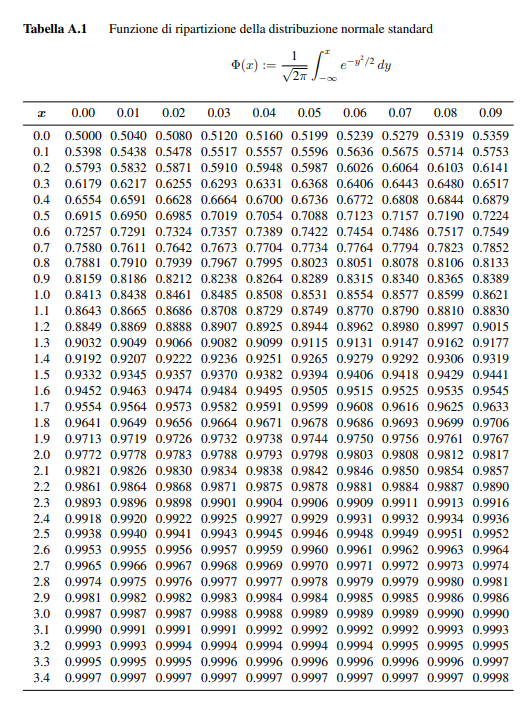
\includegraphics[width=\textwidth]{images/phi_table.png}
        \end{minipage}
        \begin{minipage}{0.4\textwidth}
            \paragraph{Esempio:} per trovare un valore \\
            se dobbiamo trovare $\boldsymbol{\Phi(1.77)}$ \\
            cerco: \\ \\
            \colorbox{bittersweet}{1.7} nelle \textit{righe} \\ \\
            \colorbox{yellow}{0.07} nelle \textit{righe}
        \end{minipage}
    \end{figure}
    \newpage
    \paragraph{$\Phi(-x)$} è possibile trovare $\Phi(-x)$ usando la \textit{simmetria della distribuzione} rispetto a 0. \\
    \begin{equation*}
        \begin{split}
            \Phi(-x) &= P(Z < -x) \\
            &= P(Z > x) \\
            &= 1 - P(Z < x) = 1 - \Phi(x) \\
        \end{split}
    \end{equation*}
    \paragraph{Esempio:}
    \[ P(Z < -1) = \Phi(-1) = 1 -\Phi(1) \approx 1 - 0.8413 \approx 0.1587 \]
    
    \paragraph{Esempio:} Sia X una variabile aleatoria normale media:$\mu = 3$, varianza:$\sigma^2 = 16$ \\
    Si trovino \textbf{(a)} P(X < 11); \textbf{(b)} P(X > -1) \textbf{(c)} P(2 < X < 7).
    \paragraph{(a)} Poniamo prima di tutto $Z := (X - \mu) / \sigma$ 
    \begin{equation*}
        \begin{split}
            P(X < 11) &= P(\frac{X - 3}{4} < \frac{11 - 3}{4}) \\
            &= P(Z < 2) \\
            &= \Phi(2) \approx 0.9972
        \end{split}
    \end{equation*}

    \paragraph{(b)} stesso ragionamento per b | (P > -1) |
    \begin{equation*}
        \begin{split}
            P(X > 1) &= P(\frac{X - 3}{4} < \frac{-1 - 3}{4}) \\
            &= P(Z > -1) \\
            &= P(Z < 1) \\
            &= \Phi(1) \approx 0.8413
        \end{split}
    \end{equation*}

    \paragraph{(c)} stesso ragionamento per c | P(2 < X < 7) |
    \begin{equation*}
        \begin{split}
            P(2 < X < 7) &= P(\frac{2 - 3}{4} < \frac{X - 3}{4} < \frac{7 - 3}{4}) \\
            &= P(-1/4 < Z < 1) \\
            &= \Phi(1) - \Phi(-0.25) \\
            &= \Phi(1) - 1 + \Phi(0.25) \approx 0.4400
        \end{split}
    \end{equation*}

    \paragraph{Riproducibilità della distribuzione normale:} Dove: \\
    $X_1, X_2 \ldots X_n$ sono \textit{aleatorie normali e indipendenti}, $X_i$ ha media $\mu_i$ e varianza $\sigma^{2}_i$ \\ \\
    La sua funzione generatrice di $\sum_{i = 1}^{n} X_i$ è data da:
    \begin{equation}
        \begin{aligned}
            \phi(t) & =E\left[\exp \left\{t X_1+t X_2+\ldots+t X_n\right\}\right] \\
            & =E\left[e^{t X_1} e^{t X_2} \ldots e^{t X_n}\right] \\
            & =\prod_{i=1}^n E\left[e^{t X_i}\right] \\
            & =\prod_{i=1}^n \exp \left\{\mu_i t+\frac{\sigma_i^2 t^2}{2}\right\} \\
            & =\exp \left\{\bar{\mu} t+\frac{\bar{\sigma}^2 t^2}{2}\right\} \longrightarrow \mathcal{N}(\overline{\mu}, \overline{\sigma}^2)
        \end{aligned}
    \end{equation}
    Dove: \\
    \begin{minipage}{0.45\textwidth}
        \[ \overline{\mu} := \sum_{i = 1}^{n} \mu_i \]
    \end{minipage}
    \begin{minipage}{0.45\textwidth}
        \[ \overline{\sigma}^2 := \sum_{i = 1}^{n} \sigma^2_i\]
    \end{minipage} \\

    \paragraph{Semplificazione:} Per ogni $\alpha \in (0,1)$ definiamo $\boldsymbol{z_a}$ in modo che:
    \[ P(Z > z_a) = 1 - \Phi(Z_a) = \alpha \] 
    Spieghiamo meglio se no non ci capiamo un cazzo. \\
    Definiamo $z_a := \Phi^{-1}(1 - \alpha)$ in modo che la probabilità che una \textit{normale standard} assuma un $z_a$ esattamente ad $\alpha$

    \paragraph{Esempio}: \\
    \begin{minipage}{0.3\textwidth}
        \[ 1 - \Phi(1.645) \approx 0.05 \]
    \end{minipage}
    \begin{minipage}{0.3\textwidth}
        \[ 1 - \Phi(1.96) \approx 0.025 \]
    \end{minipage}
    \begin{minipage}{0.3\textwidth}
        \[ 1 - \Phi(2.33) \approx 0.01 \]
    \end{minipage} \\ \\
    Diventano uguali a: \\
    \begin{minipage}{0.3\textwidth}
        \[ z_{0.05} \approx (1.645) \]
    \end{minipage}
    \begin{minipage}{0.3\textwidth}
        \[ z_{0.025} \approx (1.96) \]
    \end{minipage}
    \begin{minipage}{0.3\textwidth}
        \[ z_{0.01} \approx (2.33) \]
    \end{minipage}

    \subsection{Esponenziali}
    \definizione Una variabile aleatoria continua la cui funzione di densità è data da 
    \begin{equation*}
        f(x) =
        \begin{cases}
            \lambda e^{-\lambda x} & \text{se } x \geq 0 \\
            0 & \text{se } x < 0
        \end{cases}
    \end{equation*}
    \centerline{per $\boldsymbol{\lambda > 0}$ si dice \textbf{\textit{esponenziale}} con parametro/intensità $\lambda$}
    \definizione L' \textit{esponenziale} rappresenta la durata di vita di un fenomeno.
    \paragraph{Postilla:} La $\boldsymbol{\lambda}$ rappresenta \textit{il tasso di decadimento} della probabilità. \\
    Ovvero la \textbf{velocità} con cui la probabilità \textit{diminuisce} al cresce del tempo. \\ 
    Più è grande $\lambda$ più velocemente la probabilità diminuisce \\ \\
    La sua \textit{funzione di ripartizione} è data da:
    \begin{equation*}
        \begin{split}
            F(x) &= P(X \leq x) \\
            &= \int_{0}^{x} \lambda e^{-\lambda y} \, dy \\
            &= 1 - e^{-\lambda x} \quad x \geq 0
        \end{split}
    \end{equation*}
    Come per gli altri modelli possiamo trovare la sua \textit{funzione generatrice dei momenti} e di conseguenza i momenti e la varianza. \\
    \begin{equation}
        \begin{aligned}
            \phi(t) & :=E\left[e^{t X}\right] \\
            & =\int_0^{\infty} e^{t x} \lambda e^{-\lambda x} d x \\
            & =\lambda \int_0^{\infty} e^{-(\lambda-t) x} d x \\
            & =\frac{\lambda}{\lambda-t}, \quad t<\lambda
        \end{aligned}
    \end{equation}
    Derivando $\phi$ otteniamo $\phi'(t)$ e $\phi''(t)$:
    \[ \phi'(t) = \frac{\lambda}{(\lambda - t)^2}\]
    \[ \phi''(t) = \frac{2\lambda}{(\lambda - t)^3}\]
    Ottenendo in questo modo i soliti valori attesi e la varianza:
    \[ \ev{X} = \phi'(0) = \frac{1}{\lambda} \]
    \[ \ev{X^2} = \phi''(0) = \frac{2}{\lambda^2} \]
    \[ Var(X) = \ev{X^2} - \ev{X}^2 = \frac{1}{\lambda^2} \]
    \centerline{Per una variabile aleatoria esponenziale $\lambda$ è il \textit{reciproco} del valore atteso}
    \centerline{e la varianza è il \textit{quadrato} di quest'ultimo.}

    \definizione La proprietà centrale della distribuzione esponenziale è la sua \textbf{assenza di memoria}
    \paragraph{Spiegazione:} spieghiamo meglio quello scritto prima. \\
    La seguente proprietà ci dice che la probabilità che un evento che si verifichi in un certo lasso di tempo \textbf{non dipende} dal tempo
    trascorso fino a quel momento \\
    ma solo dal tempo trascorso a partire da quel momento. \\ \\
    In termini di formula riferendoci ad una variabile aleatoria X intendiamo che:
    \[ P(X > s + t | X > t) = P(X > s) \quad \forall s,t \geq 0 \]

    \paragraph{Esempio:} il numero di miglia percorse da una macchina prima che la batteria si scarichi è di media \textit{10.000} miglia \\
    Se una persona fa un viaggio di \textit{5.000} miglia \\
    Quale è la probabilità che lo porti a termine senza dover sostituire la batteria? e se la distribuzione non è esponenziale? \\
    - ricordandoci la proprietà \textit{di assenza di memoria della distribuzione esponenziale} il tempo di vita residuo è esponenziale \\
    con intensità $\boldsymbol{\lambda = 1 / 10}$ e quindi la probabilità cercata è: \\ \\
    \begin{equation*}
        \begin{split}
            P(\text{vita residua} > 5) &= 1 - F(5) \\
            &= e^{-5\lambda} \\
            &= e^{-0.5} \approx 0.607
        \end{split}
    \end{equation*}
    Se non avessimo saputo che la distribuzione è esponenziale, la probabilità sarebbe stata da questa equazione:
    \begin{equation*}
        \begin{split}
            P(\text{vita residua} > 5) &= P(\text{vita totale} > t + 5 | \text{vita totale} > t) \\
            &= \frac{1 - F(t + 5)}{1 - F(t)}
        \end{split}
    \end{equation*}
    \paragraph{Postilla:} \textit{t} è il numero di miglia della batteria fino al momento del viaggio \\
    Quindi senza l'informazione che la nostra distribuzione è esponenziale avremmo \textbf{bisogno di ulteriori informazioni}.


    \paragraph{Proprietà con condizione in assenza di memoria:}
    \[ \frac{P(X > s + t, X > t)}{P(X > t)} = P(X > s) \]
    e quindi anche a:
    \[ P(X > s + t) = P(X > s) P(X > t) \]
    \paragraph{Dimostrazione:}
    \[ P(X > x) = e^{-\lambda x} \rightarrow e^{-\lambda(s+t)} = e^{-\lambda s} e^{-\lambda t} \]

    \paragraph{Proposizione:} se abbiamo $X_1, X_2, \ldots X_n$ \textit{indipendenti} di parametri $\lambda_1, \lambda_2, \ldots \lambda_n$ \\
    La variabile aleatoria: \\
    $Y := min(X_1, X_2, \ldots, X_n)$ è \textbf{esponenziale} di parametro $\sum_{i = 1}^{n} \lambda_i$ \\
    \paragraph{Spiegazione:} Basta dimostrare che $\boldsymbol{P(Y \leq x) = 1 - exp\{-x \sum_{i = 1}^{n} \lambda_i \}}$ \\
    quindi che $P(Y > x) = exp\{-x \sum_{i = 1}^{n} \lambda_i \}$ \\ 
    e ora la vera dimostrazione che tanto è inutile diomerda.

    \paragraph{Dimostrazione:}
    \begin{equation}
        \begin{aligned}
            P(Y>x) & =P\left(\min \left(X_1, X_2, \ldots, X_n\right)>x\right) \\
            & =P\left(X_1>x, X_2>x, \ldots, X_n>x\right) \\
            & =\prod_{i=1}^n P\left(X_i>x\right) \quad \text { per l'indipendenza } \\
            & =\prod_{i=1}^n\left(1-F_{X_i}(x)\right) \\
            & =\prod_{i=1}^n e^{-\lambda_i x} \\
            & =e^{-x \sum_{i=1}^n \lambda_i}
        \end{aligned}
    \end{equation}
    \subsection{Processi stocastici (Poisson)}
    \definizione Famiglia di variabili aleatorie parametrizzate da un indice (in questo caso \textbf{t})
    \definizione Consideriamo una serie di eventi instantanei che avvengono però a intervalli di tempo \textbf{random} \\
    Sia $N(t)$ il numero di quanti eventi se ne sono verificati nell'intervallo $[0, t]$ \\
    $N(t)$ viene detto \textbf{processo di Poisson} di intensità $\lambda, \lambda > 0$
    \paragraph{Condizioni:}
    \begin{enumerate}
        \item $N(0) = 0 \longrightarrow$ si iniziano a contare gli eventi dal \textbf{tempo 0}
        \item Il numero degli eventi che hanno luogo in intervalli di tempo \textit{disgiunti} sono \textbf{indipendenti}. $\rightarrow$ \textit{indipendenza degli incrementi} | 
        il numero di eventi fino al tempo $t$ -> $N(t)$ è \textbf{indipendente} dal numero di eventi tra il tempo $t$ e il tempo $t+s$
        \item La distribuzione del numero degli eventi in un dato intervallo di tempo dipende dalla \textbf{lunghezza} dell'intervallo $\rightarrow$ \textit{stazionarietà degli incrementi} | la \textit{distribuzione} di $N(t+s) - N(t)$ è \textbf{la stessa} per tutti i valori di $t$
        \item $\displaystyle \lim_{h \to 0} \frac{P(N(h) = 1)}{h} = \lambda \rightarrow$ Per un intervallo di tempo \textit{molto piccolo} c'è una probabiltà di $\lambda_h$ che si \textbf{verifica un solo evento}
        \item $\displaystyle \lim_{h \to 0} \frac{P(N(h) \geq 2)}{h} = 0 \rightarrow$ Per un intervallo di tempo \textit{molto piccolo} c'è una probabiltà \textbf{nulla} che se ne verifichino due o più.
    \end{enumerate}
    Con queste ipotesi qua di sopra è possibile dimostrare che \textit{il numero di eventi} che si verificano in un qualsiasi intervallo di tempo $t$ è una \textit{variabile aleatoria di Poisson} di media $\lambda_t$. \\
    \textbf{Se $n$ è grande:}
    \[ P(N(t) = k) \approx P(k \text{ sottointervalli con 1 evento, n-k con 0 eventi}) \]
    \centerline{Sempre per n grande, la condizione \textbf{4} e le condizioni \textbf{4} e \textbf{5} insieme implicano che:}
    \[ P(1 \text{ evento in un sottointervallo fissato}) \approx \frac{\lambda_t}{n} \]
    \[ P(0 \text{ eventi in un sottointervallo fissato}) \approx 1 - \frac{\lambda_t}{n} \]
    Utilizzando l'indipendenza della condizione 2 (\textit{indipendenza degli incrementi}) il numero totale di eventi
    è assimilabile ad una variabile aleatoria \textbf{binomiale}.
    \[ P(k \text{ sotto intervalli con 1 evento, n - k con eventi}) \approx \binom{n}{k} (\frac{\lambda_t}{n})^k (1 - \frac{\lambda_t}{n})^{n-k}  \] 
    \centerline{Se $n$ tende all'infinito può essere \textit{approssimata con Poisson} media $\lambda_t$}
    \[ P(N(t) = k) \approx \frac{(\lambda t)^k}{k!} e^{-\lambda t}\]

    \paragraph{Proposizione} Siano $X_1, X_2, \cdots X_n$ intervalli di tempo che intercorrono rispettivamente dal 1' al 2' al 3' ecc. \\
    \paragraph{Esempio:} $X_1 = 5$ e $X_2 = 8$ il primo evento avviene all'istante \textit{5} e il secondo all'istante \textit{13} (5+8) \\
    Vogliamo determinare la distribuzioni delle $X_i$ (ricordando che l'evento $\{X_1 > t\}$ si verifica se nell'intervallo [0, t] \textit{non si sono realizzati eventi}) quindi:
    \[ P(X_1 > t) = P(N(t) = 0) = e^{\lambda t} \]
    \centerline{Questo significa che:}
    \[ F_{X_1}(t) := P(X_1 \leq t) = 1 - e^{-\lambda t} \]
    $X_i$ è una variabile aleatoria \textit{esponenziale} di intensità $\lambda$ \\
    Per trovare $X_2$ si noti che qualunque valore $s$ assuma la variabile aleatoria $X_1$ è data da:
    \begin{equation*}
        \begin{split}
            P(X_2 > t | X_1 = s) &= P(0 \text{ eventi in} (s, s + t | X_1 = s)) \\
            &= P(0 \text{ eventi in} (s, s + t )) \quad \text{per la condizione \textbf{2}} \\
            &= e^{-\lambda t}
        \end{split}
    \end{equation*}
    Questo prova che la variabile aleatoria $X_1$ è \textbf{esponenziale} \\
    e $X_2$ è esponenziale di intensità $\lambda$ e \textbf{indipendente} da $X_1$ \\
    \paragraph{Proposizione:} Le $X_i$ sono tutte \textit{variabili esponenziali} \\
    quindi i tempi che separano gli eventi di Poisson di intensità $\lambda$ \\
    sono una \textit{successioni di esponenziali indipendenti} 

    \subsection{Gamma}
    \definizione Una variabile aleatoria \textit{continua} si dice distribuzione di \textit{tipo gamma}
    di parametri $(\alpha, \lambda)$ con $\alpha > 0$ e $\lambda > 0$ la sua funzione di intensità è data da:

    \begin{equation*}
        f(x) =
        \begin{cases}
            \frac{\lambda^\alpha}{\Gamma(\alpha)} x^{\alpha - 1} e^{-\lambda x} & \text{se } x > 0 \\
            0 & \text{se } x \leq 0 
        \end{cases}
    \end{equation*}
    dove con $\boldsymbol{\Gamma}$ indichiamo la funzione \textit{gamma di Eulero}, definita in modo da normalizzare l'integrale di f come segue:
    \begin{equation}
        \begin{aligned}
            \Gamma(\alpha) & :=\int_0^{\infty} \lambda^\alpha x^{\alpha-1} e^{-\lambda x} d x \\
            & =\int_0^{\infty} y^{\alpha-1} e^{-y} d y \quad \text { ponendo } y=\lambda x
        \end{aligned}
    \end{equation}
    è possibile \textbf{integrare} per parti, se $\boldsymbol{\alpha > 1}$ possiamo scrivere:
    \begin{equation}
        \begin{aligned}
            \int_0^{\infty} y^{\alpha-1} e^{-y} d y & =-\left.y^{\alpha-1} e^{-y}\right|_{y=0} ^{\infty}+\int_0^{\infty}(\alpha-1) y^{\alpha-2} e^{-y} d y \\
            & =(\alpha-1) \int_0^{\infty} y^{\alpha-2} e^{-y} d y
        \end{aligned}
    \end{equation}
    Dove il termine $-y^{a-1} e^{-y} \bigg\rvert_{y = 0}^{\infty}$ è \textbf{nullo} perche $\boldsymbol{\alpha > 1}$ implica che $\lim_{y \to 0} y^{\alpha - 1} = 0$

    \subsection{Chi-quadro}

    \subsection{Distribuzione T}

    \subsection{Distribuzione F}

    \subsection{Distribuzione logistica}

\end{document}